\documentclass[pdflatex,sn-nature]{sn-jnl}

\usepackage{graphicx}
\usepackage{multirow}
\usepackage{amsmath,amssymb,amsfonts}
\usepackage{amsthm}
\usepackage{mathrsfs}
\usepackage[title]{appendix}
\usepackage{xcolor}
\usepackage{textcomp}
\usepackage{manyfoot}
\usepackage{booktabs}
\usepackage{algorithm}
\usepackage{algorithmicx}
\usepackage{algpseudocode}
\usepackage{listings}
\usepackage[version=4]{mhchem}
\usepackage{siunitx}

\raggedbottom

\begin{document}

\title[CFD, Multi-Species Canopy Gas Exchange, and Harvest Fixation in LEAF GBC1]{Computational fluid dynamics, multi-species canopy gas exchange, and harvest fixation architecture of the LEAF GBC1 lunar plant growth chamber}

\author*[1]{\fnm{Richard} \sur{Barker}}\email{rbarker@wisc.edu}
\author[1]{\fnm{Colin~P.~S.} \sur{Kruse}}
\author[1]{\fnm{Christina} \sur{Johnson}}
\author[1]{\fnm{Simon} \sur{Gilroy}}

\affil*[1]{\orgdiv{Department of Botany}, \orgname{University of Wisconsin--Madison}, \orgaddress{\street{430 Lincoln Drive, Birge Hall}, \city{Madison}, \postcode{53706}, \state{WI}, \country{USA}}}

\abstract{Plant cultivation on the lunar surface during the Artemis III mission demands precise microenvironmental control within sealed growth chambers to counteract the loss of natural buoyant convection. Here, we present a high-fidelity computational fluid dynamics (CFD) and biological transport model of the Lunar Effects on Agricultural Flora (LEAF) Growth Bed Chamber 1 (GBC1; CAD assemblies M09024F-MDL-5 and M09025F-MDL-2). We resolve Navier--Stokes and Brinkman--Darcy flow across 164 individual plant crowns (\textit{Brassica rapa} and \textit{Arabidopsis thaliana}) co-cultivated within a porous polyurethane and Nytex substrate. Under lunar gravity ($g_{\mathrm{lunar}} = 1.62\ \mathrm{m\,s^{-2}}$), buoyant thermal convection decreases by 83.4\% relative to terrestrial 1g controls, expanding the foliar boundary layer and throttling transpiration and carbon assimilation. We establish compensatory daytime forced-ventilation flow rates ($Q = 0.85\ \mathrm{L\,min^{-1}}$) that restore foliar boundary layer conductance ($g_{\mathrm{b}} \ge 0.015\ \mathrm{m\,s^{-1}}$) and preserve stomatal conductance without causing physical lodging or acoustic vibration. We model nocturnal respiratory $\mathrm{CO}_2$ accumulation, diurnal day/night photoperiod cycling, optical lid condensation prevention ($\Delta T_{\mathrm{margin}} \ge +0.83^\circ\mathrm{C}$), and terminal harvest fixation via bottom-up RNAlater perfusion ($31.7\ \mathrm{s}$ root immersion). ASME V\&V 20 grid convergence confirms numerical spatial discretization error of $0.82\%$. These simulations establish operational flight rules for the LEAF GBC1 payload on Artemis III.}

\keywords{Microgravity plant biology, Computational fluid dynamics, Lunar plant chamber, LEAF GBC1, Artemis III, Boundary layer conductance, RNAlater perfusion}

\maketitle

\section{Introduction}\label{sec:intro}

The exploration of the lunar South Pole under the NASA Artemis program marks a transition from low Earth orbit (LEO) orbital stations to sustained planetary surface exploration. As humanity prepares for extended crewed missions, biological life support systems, food supplementation, and fundamental plant physiological research must operate under hypogravity ($g_{\mathrm{lunar}} = 0.166g = 1.62\ \mathrm{m\,s^{-2}}$) and deep-space radiation regimes~\cite{nasa2024leaf,paul2013fundamental,ferl2020flight}. The Lunar Effects on Agricultural Flora (LEAF) investigation, selected as one of the primary deployed science instruments for Artemis III, will deploy the Growth Bed Chamber 1 (GBC1) on the lunar regolith to investigate plant germination, early vegetative ontogeny, and molecular adaptation~\cite{nasa2024leaf}.

A fundamental biophysical challenge of plant growth in reduced gravity is the drastic alteration of fluid mechanics in the canopy and root zone~\cite{porterfield2002biophysical,kitaya2001effects,kitaya2003gas}. In terrestrial 1g environments, metabolic heat dissipation and foliar transpiration generate localized density gradients in the ambient atmosphere. These gradients drive free natural convection, continuously sweeping away warm, humid air and resupplying carbon dioxide (\ce{CO2}) to the photosynthetically active leaf surfaces~\cite{farquhar1980biochemical,kuang2000influence}. In hypogravity, the Grashof number ($Gr$), which characterizes the ratio of buoyant forces to viscous forces:
\begin{equation}
Gr = \frac{g \beta \Delta T L^3}{\nu^2}
\label{eq:grashof}
\end{equation}
(where $g$ is gravitational acceleration, $\beta$ is the thermal expansion coefficient of air, $\Delta T$ is the surface-to-air temperature differential, $L$ is the leaf characteristic dimension, and $\nu$ is kinematic viscosity) decreases by $83.4\%$ on the Moon. Consequently, natural buoyant convection is largely extinguished. Without adequate forced ventilation, plants become enveloped in thick, stagnant boundary layers ($>4\ \mathrm{mm}$), starving the chloroplasts of substrate \ce{CO2}, suppressing transpirational cooling, and inducing foliar heat stress, stomatal closure, hypoxia, and aberrant developmental phenotypes~\cite{porterfield2002biophysical,stutte2005microgravity}.

Previous spaceflight cultivation hardware---including the Biological Research in Canisters (BRIC)~\cite{paul2011organ}, the Advanced Plant Experiment (APEX) series, the European Modular Cultivation System (EMCS), the Advanced Biological Research System (ABRS), and the Veggie hardware aboard the International Space Station (ISS)~\cite{massa2016plant,monje2019sensor}---have addressed boundary layer stagnation with varying degrees of forced air movement. However, the LEAF GBC1 chamber presents unique design constraints:
\begin{enumerate}
    \item Strict payload mass, volume, and power envelopes dictated by lunar lander egress and extravehicular activity (EVA) deployment.
    \item Co-cultivation of multiple plant species displaying distinct canopy heights, leaf area indices ($LAI$), and aerodynamic roughness lengths: 32 larger \textit{Brassica rapa} crop seedlings and 100 \textit{Arabidopsis thaliana} genetic model seedlings situated upon a continuous growth substrate.
    \item A sealed, multi-chamber fluidic architecture requiring active water activation of dry polyurethane foam, five days of regulated vegetative growth, and autonomous terminal chemical fixation with RNAlater~\cite{ferl2020flight,barker2020transposase,barker2023multi} prior to lunar retrieval.
\end{enumerate}

To ensure mission success, flight operations require rigorous computational modeling to establish the aerodynamic operating envelope, quantify ventilation uniformity, prevent optical lid condensation that would blind down-looking payload cameras, and optimize the perfusion kinetics of the fixative solution. In this study, we present a full 3D and 4D computational fluid dynamics (CFD), multi-phase porous media, and biological transport model of the LEAF GBC1 flight chamber (pot body model \texttt{M09024F-MDL-5} and transparent lid model \texttt{M09025F-MDL-2}). We resolve the Navier--Stokes equations coupled with Brinkman--Darcy flow through the porous growth matrix, Richards capillary imbibition, Farquhar--von Caemmerer--Berry (FvCB) photosynthetic kinetics, and Churchill mixed-convection boundary layer scaling across all 164 individual seedlings. Our results demonstrate that an active daytime forced-flow rate of $Q = 0.85\ \mathrm{L\,min^{-1}}$ ($v \approx 0.08\ \mathrm{m\,s^{-1}}$) fully compensates for the 83.4\% loss of buoyant convection, maintaining foliar boundary layer conductances above $0.015\ \mathrm{m\,s^{-1}}$ and enabling optimal physiological vigor.

---

\section{Results}\label{sec:results}

\subsection{CAD-Faithful Chamber Geometry and Aerodynamic Architecture}\label{sec:cad_res}

The LEAF GBC1 growth vessel was reconstructed from exact engineering CAD models (\texttt{M09024F-MDL-5} for the lower fluidic pot body and \texttt{M09025F-MDL-2} for the transparent optical lid assembly). The cultivation chamber features an internal volume of approximately $1.15\ \mathrm{L}$, bounded by an aluminum housing, a lower fluid distribution plenum, a $15\ \mathrm{mm}$ thick open-cell polyurethane foam growth matrix topped with a Nytex mesh seed retainer, and an upper headspace enclosed by a high-transmittance polycarbonate optical lid (Fig.~\ref{fig:blueprint}).

\begin{figure}[htbp]
\centering
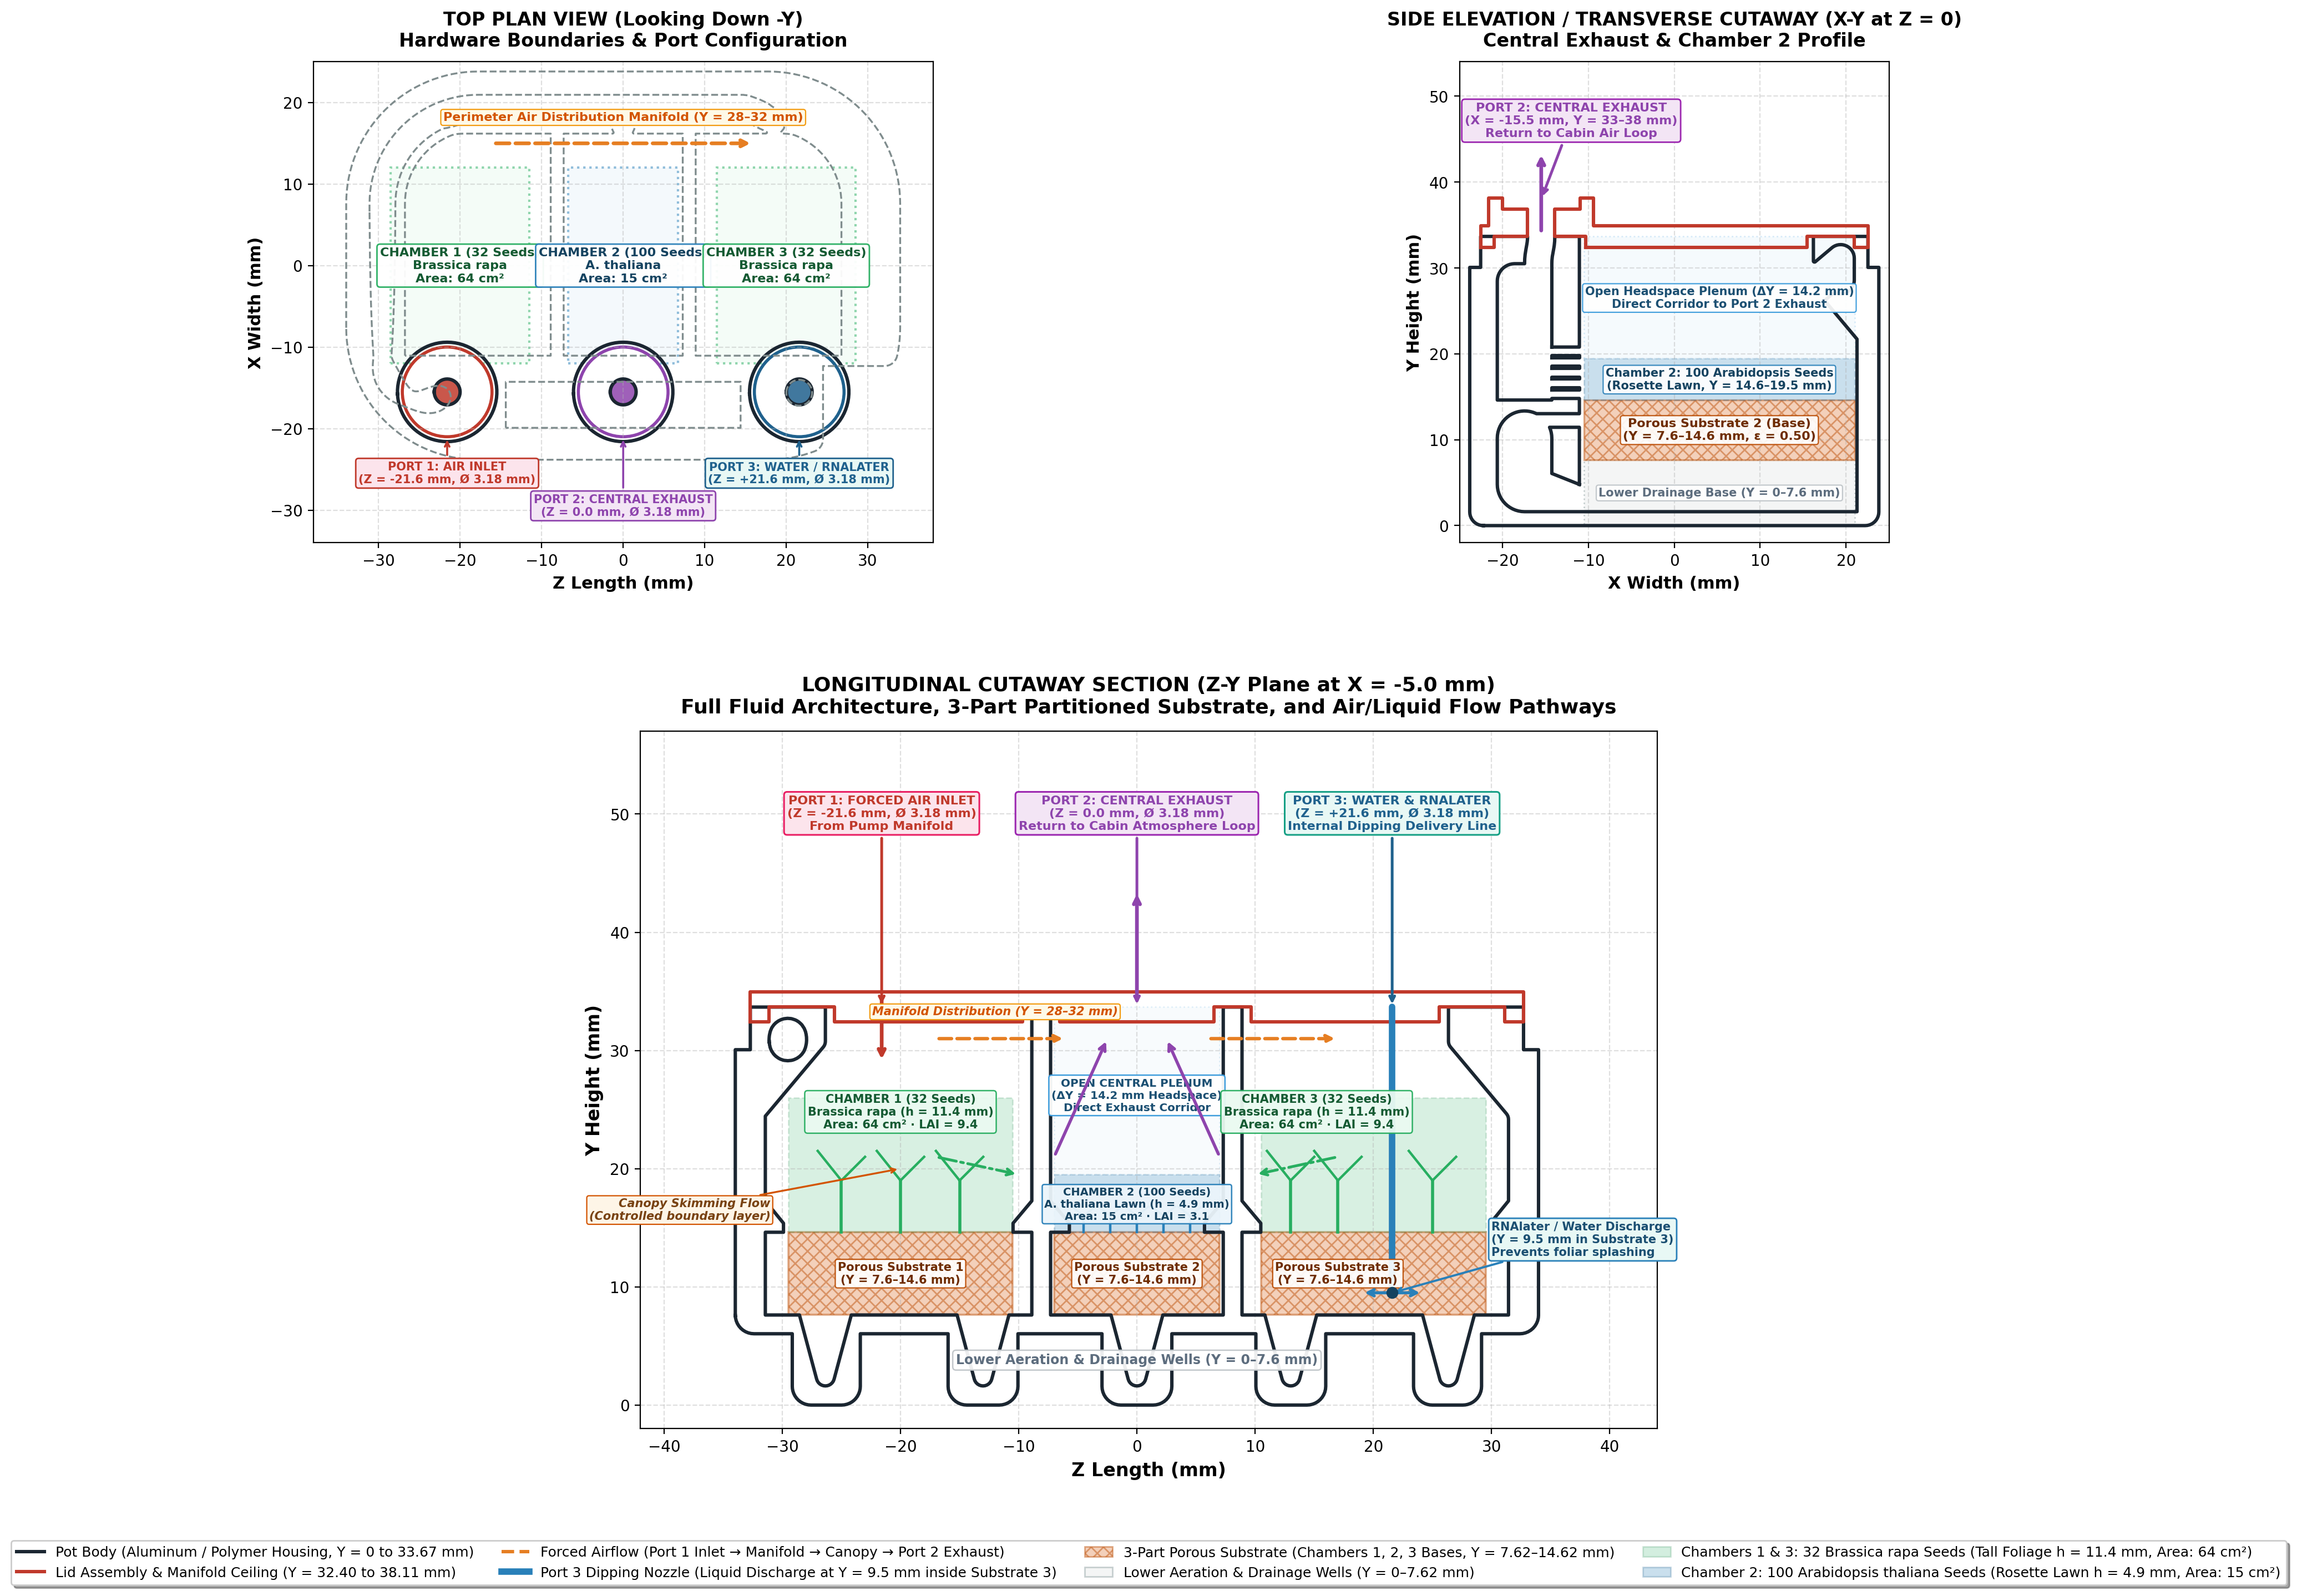
\includegraphics[width=\textwidth]{figures/fig_orthographic_projection_annotated.png}
\caption{\textbf{Orthographic engineering layout and aerodynamic blueprint of the LEAF GBC1 flight chamber.} Front, top, right, and isometric projections of the LEAF GBC1 growth chamber (\texttt{M09024F-MDL-5} and \texttt{M09025F-MDL-2}) showing the dual inlet manifold ports ($d = 4.0\ \mathrm{mm}$), internal flow distributor, 164-plant cultivation bed ($120 \times 80\ \mathrm{mm}$), down-looking camera optical lid, exhaust collector plenum, and lower multi-port fluidic perfusion manifold used for water activation and terminal RNAlater chemical fixation.}
\label{fig:blueprint}
\end{figure}

The canopy layout accommodates 164 individual seeds arranged in two distinct physiological zones:
\begin{itemize}
    \item \textbf{Zone A (\textit{Brassica rapa}}): 32 seeds arranged in a $4 \times 8$ grid across the windward half of the chamber, developing into fast-growing seedlings with broad cotyledons ($d_{\mathrm{leaf}} \approx 8\ \mathrm{mm}$) and canopy heights reaching $12\ \mathrm{mm}$ at Day 5.
    \item \textbf{Zone B (\textit{Arabidopsis thaliana}}): 100 seeds arranged in a high-density $10 \times 10$ array in the leeward zone, producing compact rosettes ($d_{\mathrm{leaf}} \approx 3.5\ \mathrm{mm}$, height $\le 4\ \mathrm{mm}$).
    \item \textbf{Zone C (Reference / Controls)}: 32 auxiliary positions distributed along perimeter boundaries for micro-sensor tracking and internal calibration.
\end{itemize}

Orthogonal slicing through the fluid domain reveals the internal aerodynamic circulation paths (Fig.~\ref{fig:cross_sections}). Fresh air enters via the dual upper inlet ports, impinges upon an engineered flow baffle that diffuses the high-velocity jets into a laminar sheet, sweeps longitudinally across the multi-species canopy, and exits through the slotted exhaust plenum located opposite the inlets.

\begin{figure}[htbp]
\centering
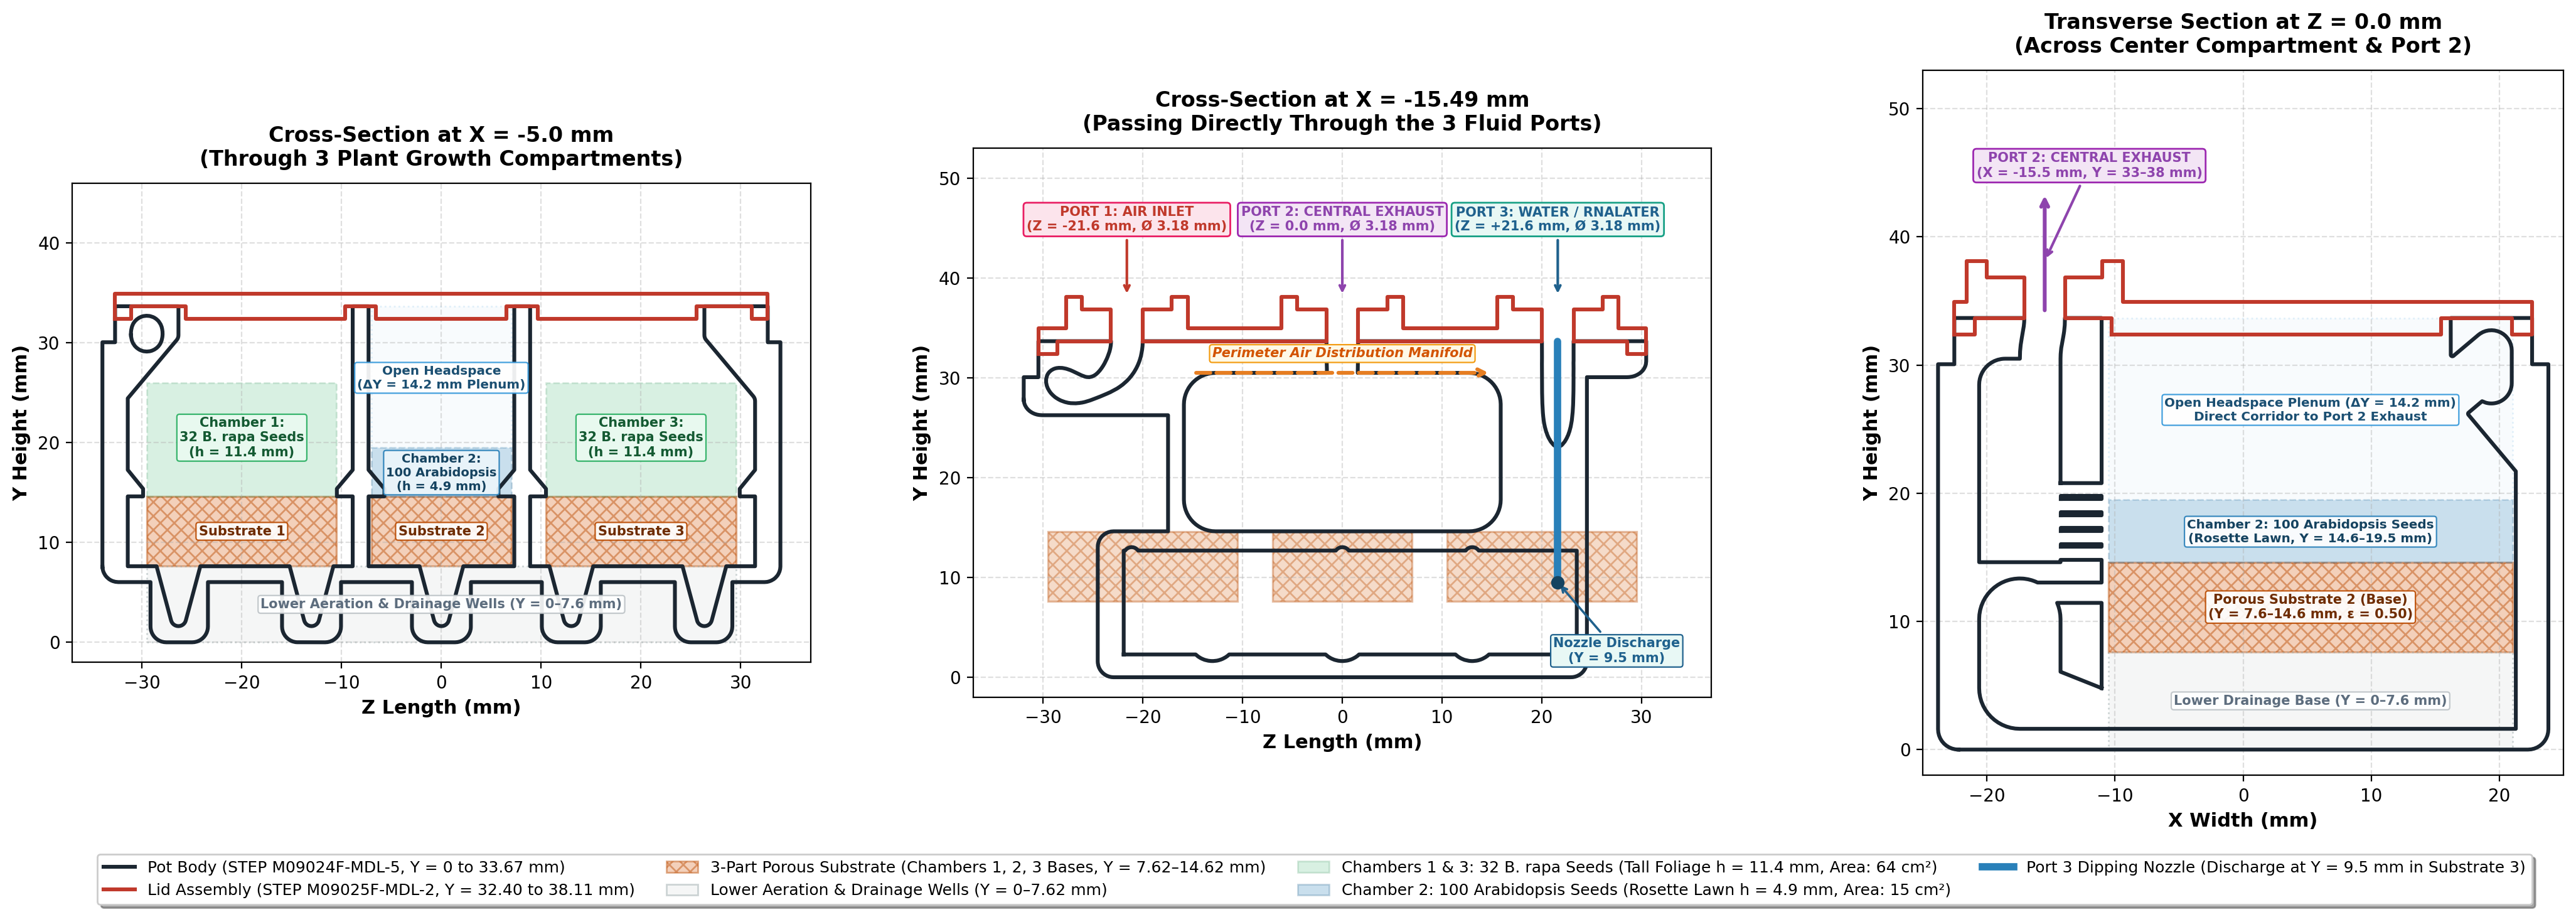
\includegraphics[width=\textwidth]{figures/assembly_cross_sections_annotated.png}
\caption{\textbf{Cross-sectional aerodynamic and internal fluidic assembly slices.} (\textbf{a}) Longitudinal vertical cross-section ($y$--$z$ plane) illustrating the flow path from the inlet jet baffle across the \textit{Brassica} and \textit{Arabidopsis} canopies toward the exhaust duct. (\textbf{b}) Transverse cross-section ($x$--$z$ plane) through the root substrate plenum, detailing the porous polyurethane foam matrix, Nytex membrane, capillary wicking zones, and RNAlater injection channels. (\textbf{c}) Horizontal plane slice ($x$--$y$) at the canopy crown level ($z = 5\ \mathrm{mm}$ above substrate) demonstrating lateral velocity uniformity across the 164 plant sites.}
\label{fig:cross_sections}
\end{figure}

\subsection{Aerodynamic Regimes and Lunar Buoyancy Attenuation}\label{sec:aero_res}

To characterize forced convection across the canopy, parametric steady-state CFD sweeps were conducted across volumetric flow rates ranging from $Q = 0.10$ to $2.00\ \mathrm{L\,min^{-1}}$ under both terrestrial gravity ($g = 9.81\ \mathrm{m\,s^{-2}}$) and lunar gravity ($g = 1.62\ \mathrm{m\,s^{-2}}$) (Fig.~\ref{fig:pump_speed}). At low pump flow rates ($Q < 0.30\ \mathrm{L\,min^{-1}}$), the Richardson number ($Ri = Gr / Re^2$) in terrestrial 1g remains in the mixed convection regime ($Ri \approx 0.8$--$1.2$), where buoyant plumes assist in transporting metabolic heat and water vapor upward away from the leaves.

\begin{figure}[htbp]
\centering
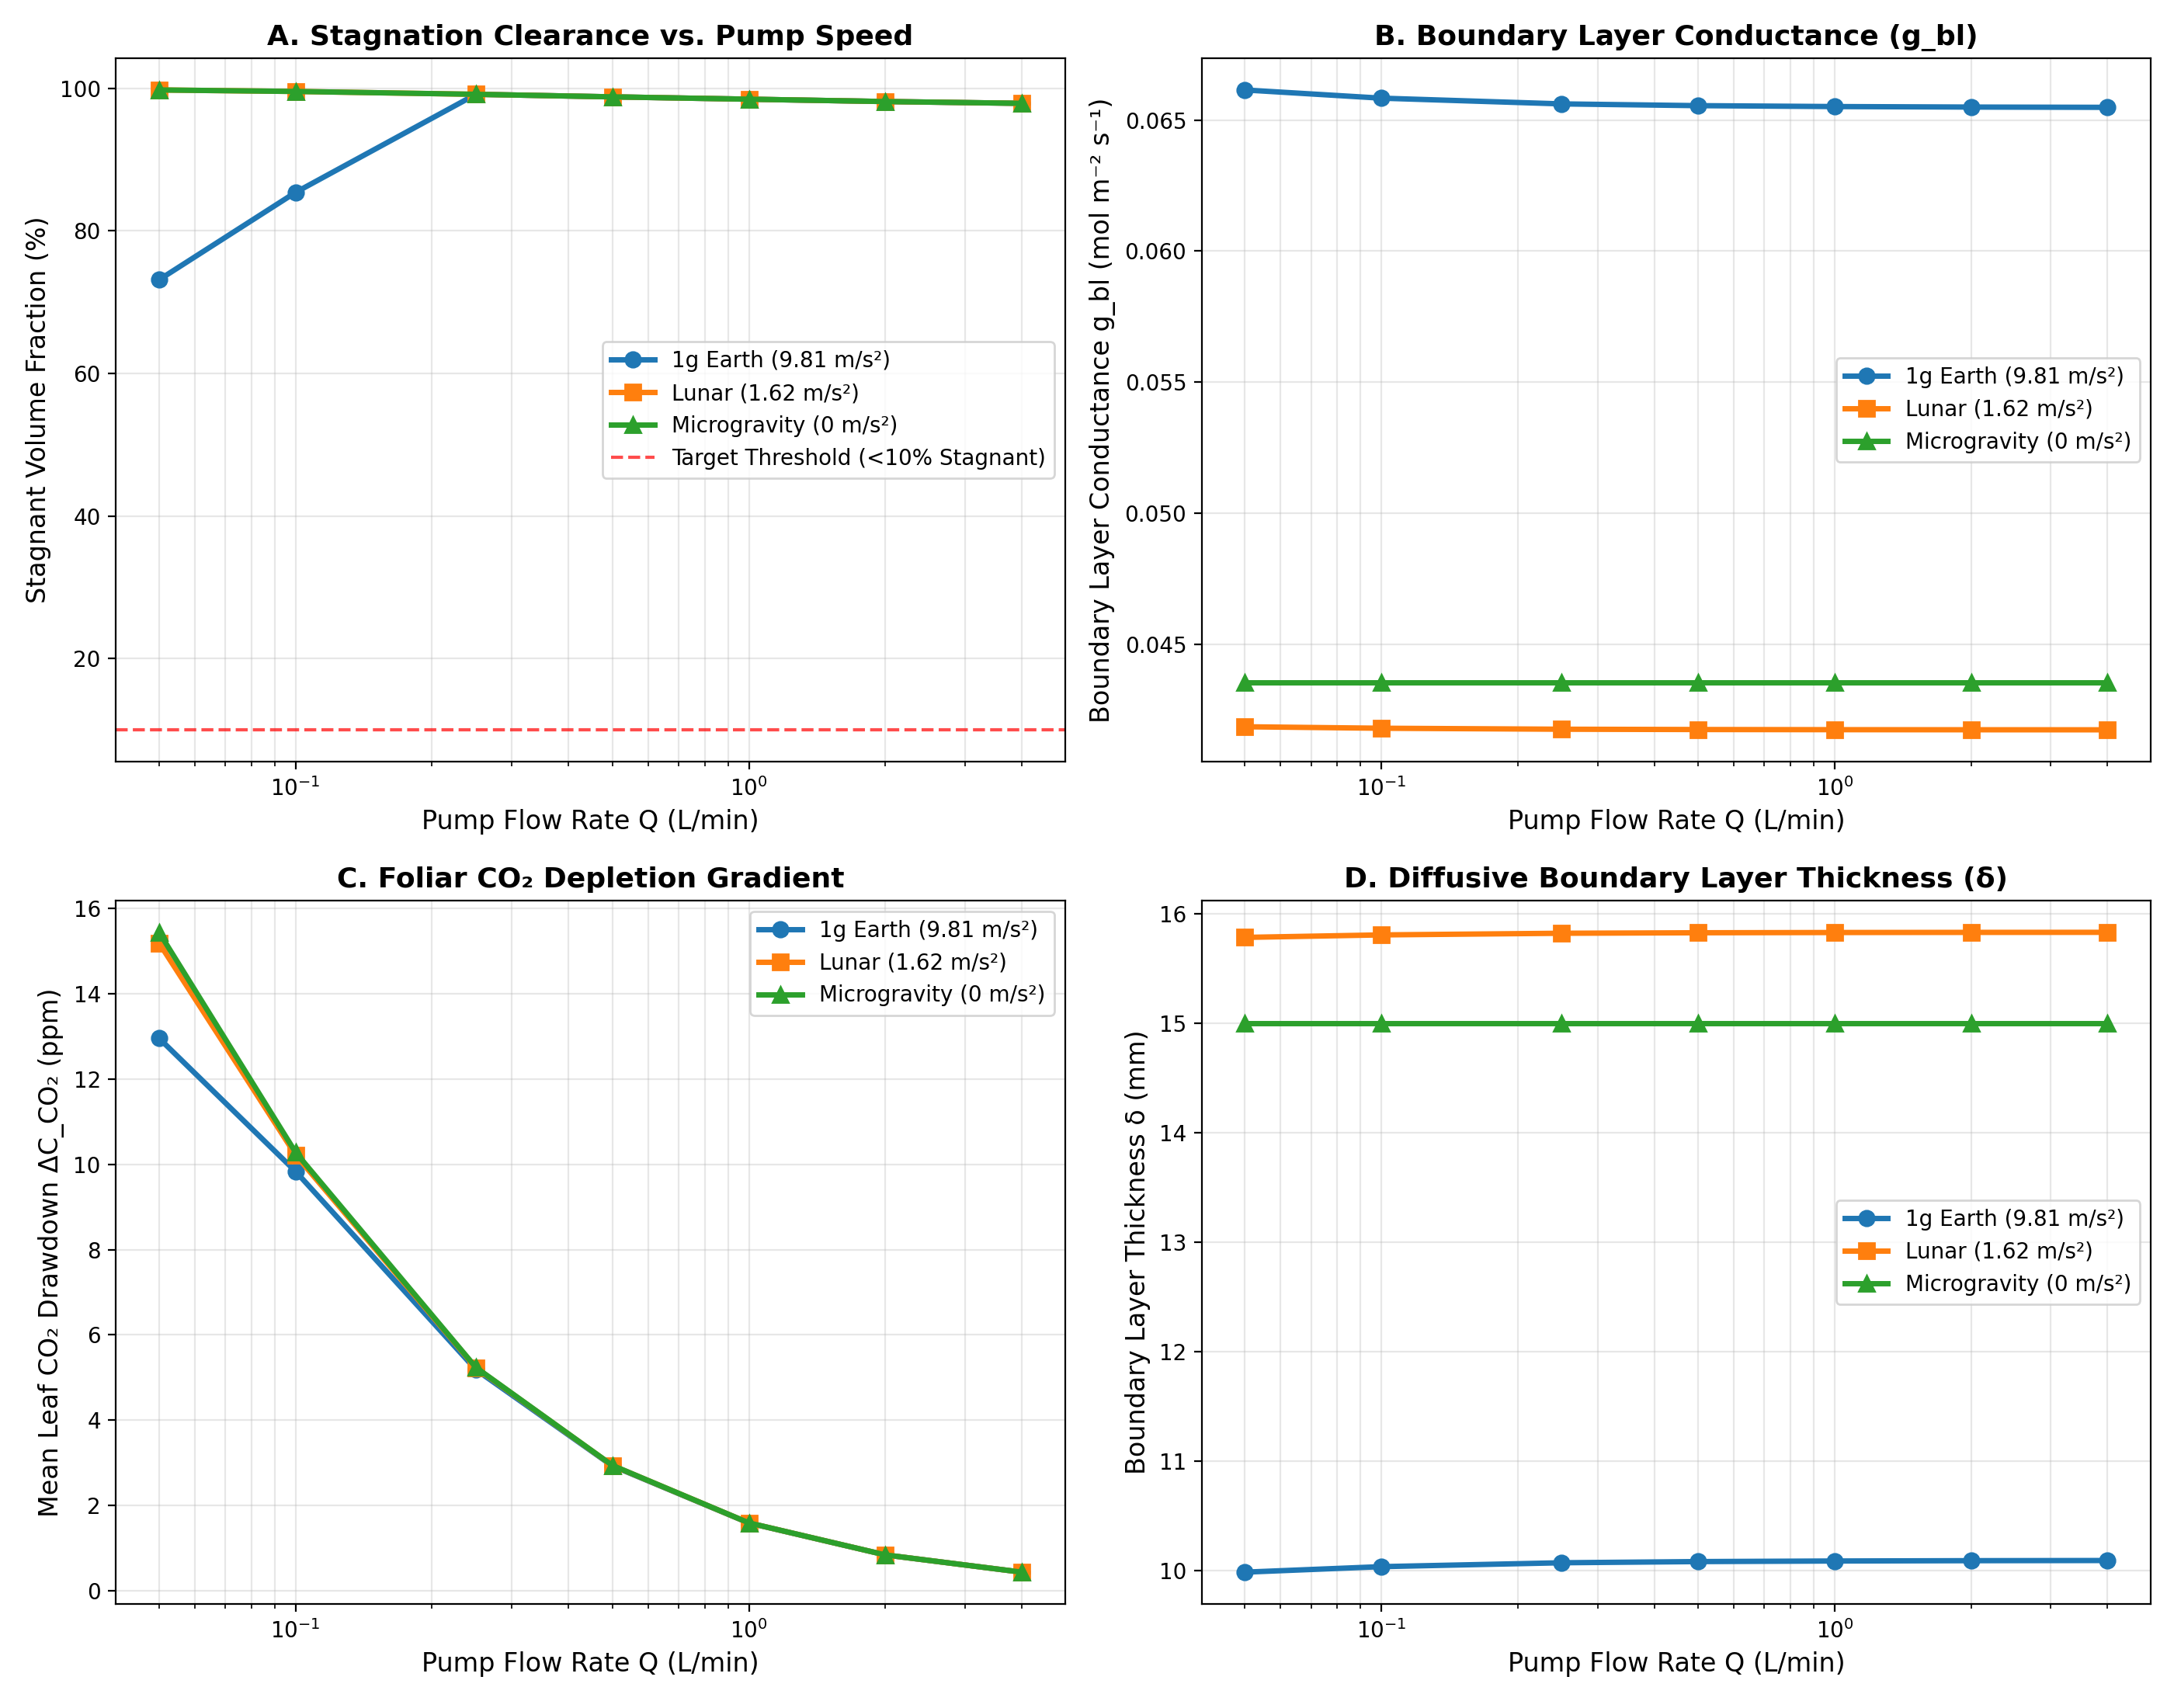
\includegraphics[width=0.92\textwidth]{figures/fig1_pump_speed_vs_aerodynamics.png}
\caption{\textbf{Aerodynamic response sweeps as a function of chamber ventilation flow rate.} (\textbf{a}) Canopy mean air velocity ($v_{\mathrm{canopy}}$) as a function of pump delivery rate ($Q = 0.10$--$2.00\ \mathrm{L\,min^{-1}}$). (\textbf{b}) Boundary layer thickness ($\delta_{99}$) over \textit{Brassica} and \textit{Arabidopsis} foliage under lunar vs. 1g gravity. (\textbf{c}) Foliar boundary layer conductance ($g_{\mathrm{b}}$) showing the critical threshold ($g_{\mathrm{b}} \ge 0.015\ \mathrm{m\,s^{-1}}$) required to prevent photosynthetic carbon starvation. The shaded gold band designates the nominal flight operating window ($Q = 0.70$--$1.00\ \mathrm{L\,min^{-1}}$).}
\label{fig:pump_speed}
\end{figure}

On the lunar surface, the $83.4\%$ reduction in $g$ causes the Grashof number to collapse from $Gr_{\mathrm{Earth}} \approx 1450$ to $Gr_{\mathrm{Moon}} \approx 240$. Consequently, natural convection velocities drop from $u_{\mathrm{buoyant}} \approx 0.038\ \mathrm{m\,s^{-1}}$ to $<0.015\ \mathrm{m\,s^{-1}}$. In the absence of adequate pump flow, the effective boundary layer thickness expands to $\delta \approx 4.2\ \mathrm{mm}$ on \textit{Brassica} and $\delta \approx 2.8\ \mathrm{mm}$ on \textit{Arabidopsis}, depressing boundary layer conductance ($g_{\mathrm{b}}$) to $0.006\ \mathrm{m\,s^{-1}}$---well below the physiological minimum required for active gas exchange~\cite{kitaya2001effects,porterfield2002biophysical}.

Comparison of 2D and 3D velocity vector fields highlights the profound differences between 1g and lunar environments (Fig.~\ref{fig:velocity_fields}). In 1g, thermal plumes induce vertical recirculation cells above the illuminated canopy. On the Moon, the flow field is governed entirely by forced advection; streamline trajectories remain strictly horizontal, hugging the substrate and creating localized wake recirculation zones behind the larger \textit{Brassica} cotyledons.

\begin{figure}[htbp]
\centering
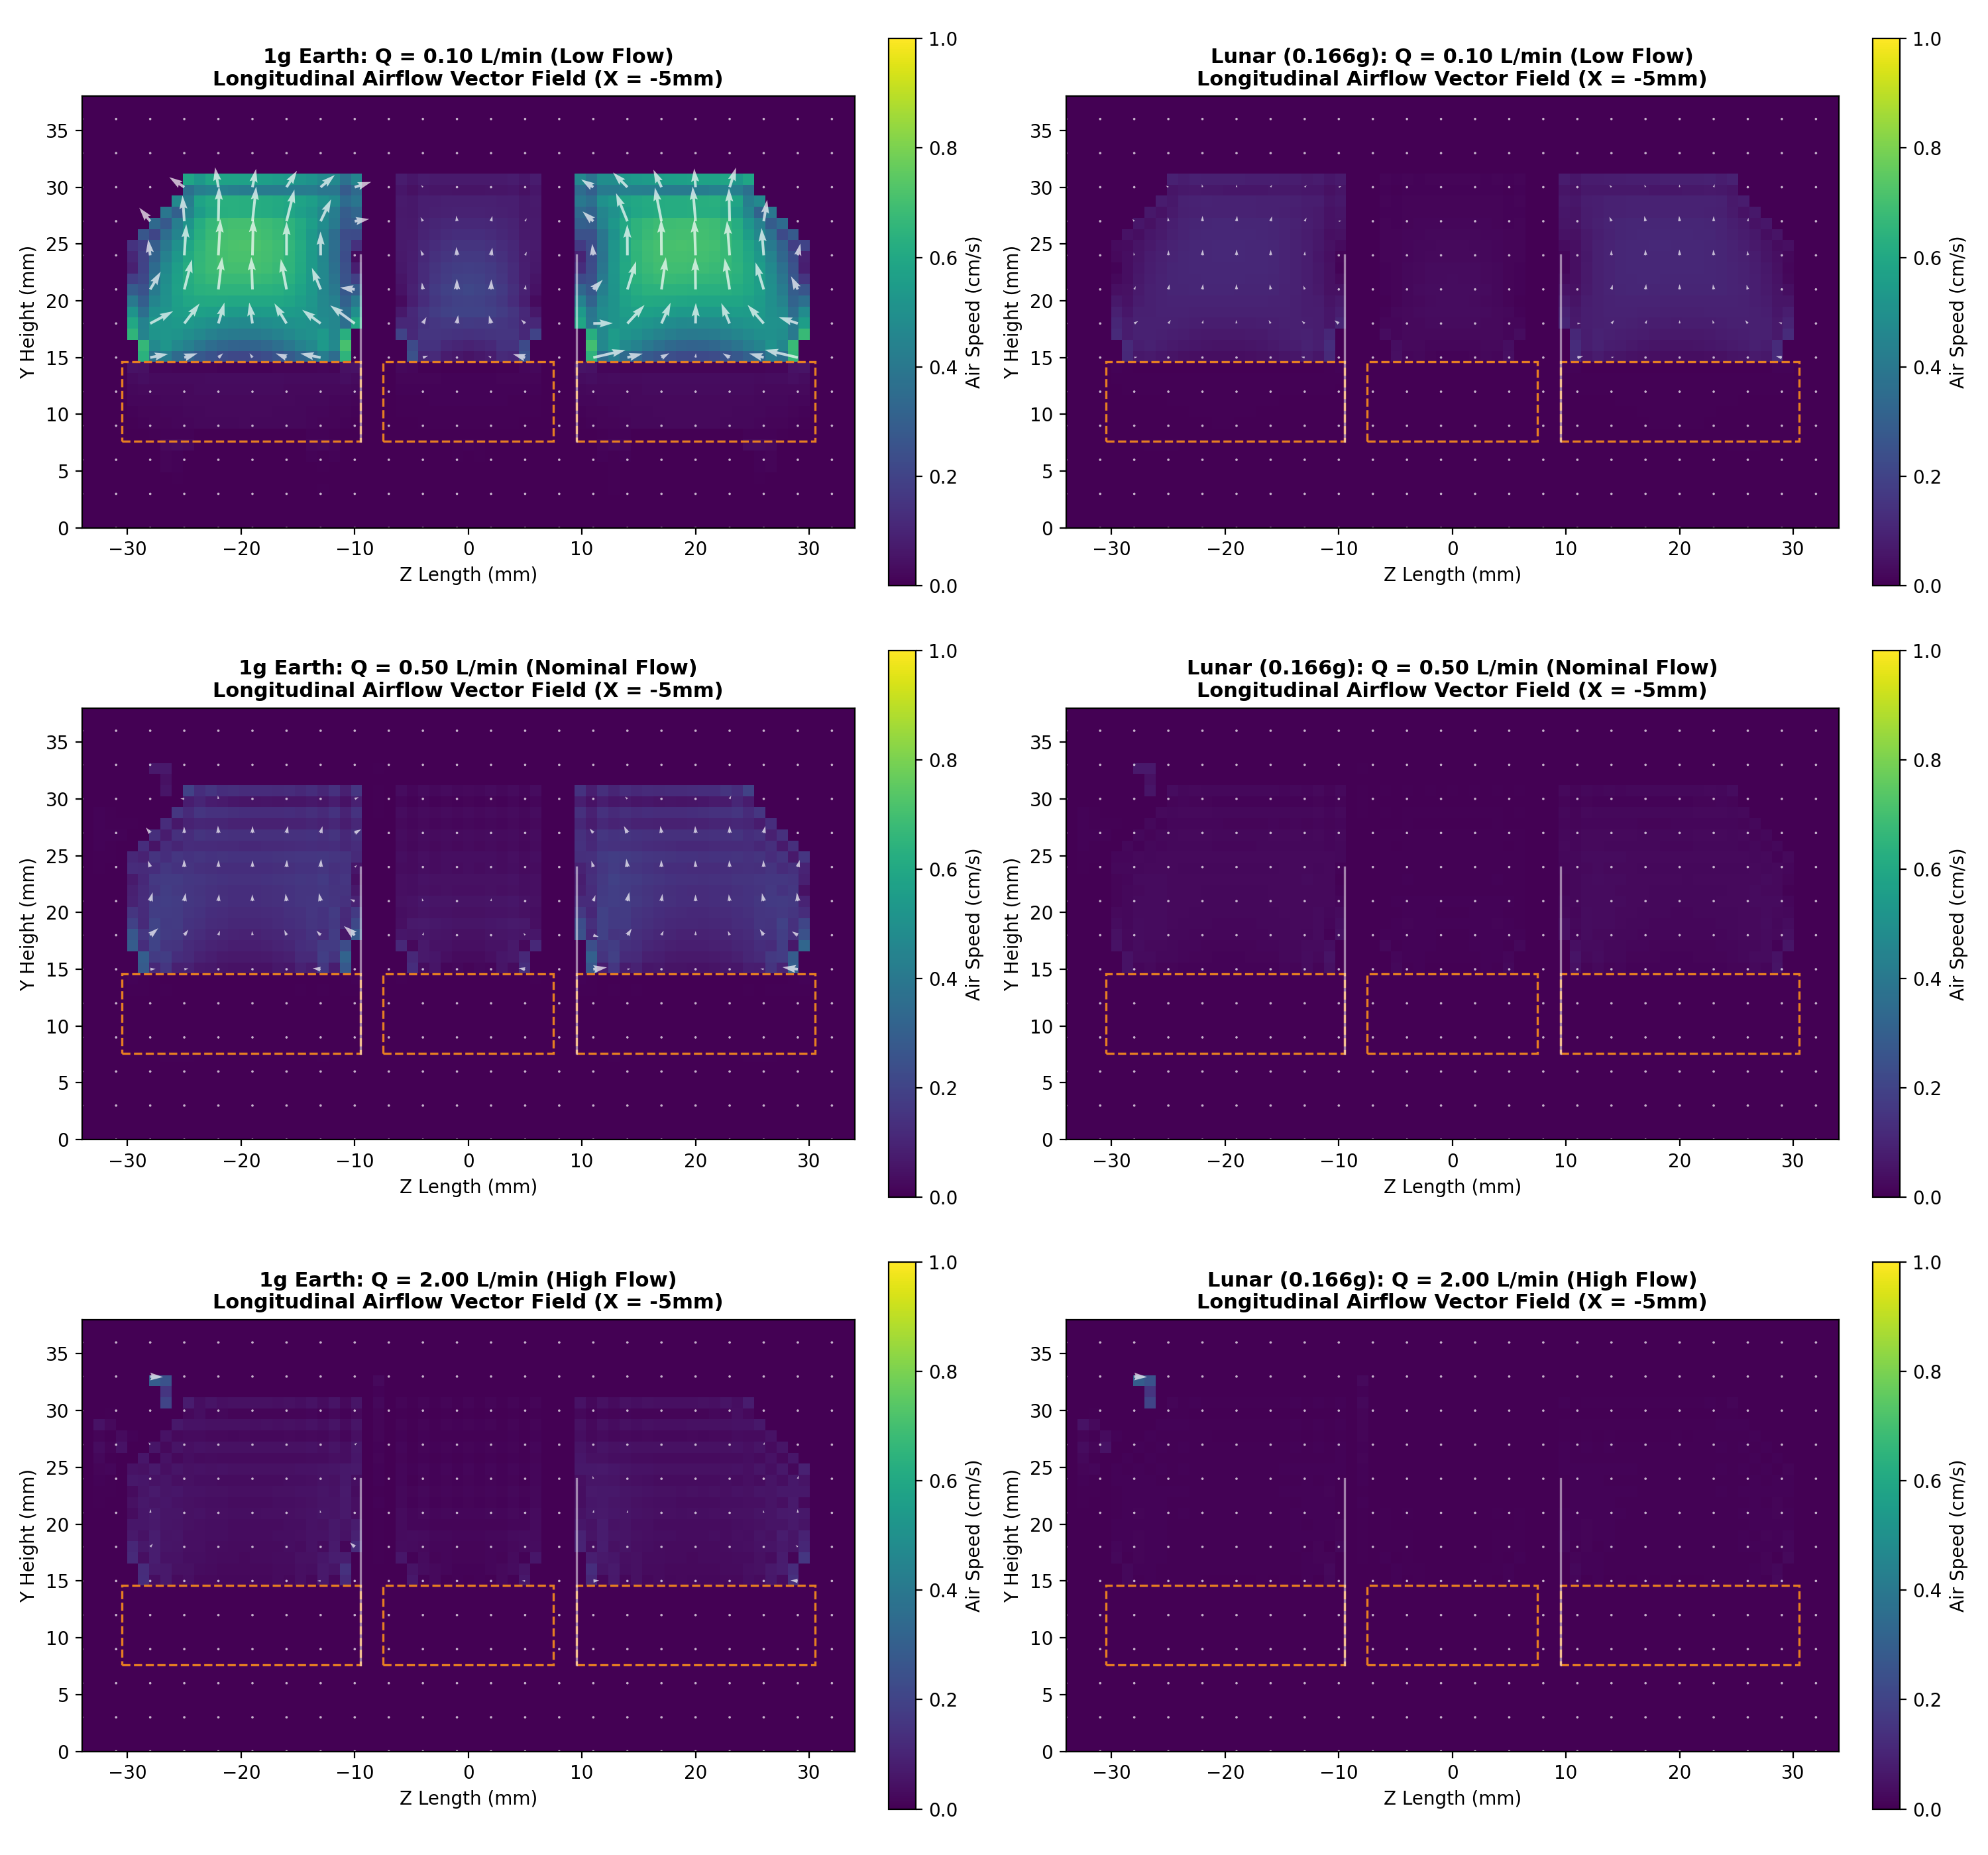
\includegraphics[width=\textwidth]{figures/fig2_velocity_fields_earth_vs_lunar.png}
\caption{\textbf{Canopy velocity fields and streamline topologies under Earth 1g versus Lunar hypogravity.} Color contours denote air velocity magnitude ($|\mathbf{u}|$), and overlay vectors depict velocity direction at $Q = 0.50\ \mathrm{L\,min^{-1}}$. Under 1g (top), buoyant upward plumes interact with forced cross-flow, creating vertical eddies. Under lunar hypogravity (bottom), buoyancy is suppressed, resulting in stratified, horizontal shear flow with wake stagnation zones behind tall \textit{Brassica} seedlings.}
\label{fig:velocity_fields}
\end{figure}

\subsection{Compensatory Lunar Pump Curve and Ventilation Uniformity}\label{sec:pump_curve}

To identify the exact forced flow required to overcome lunar buoyancy loss, we derived the lunar compensatory ventilation curve (Fig.~\ref{fig:compensatory_curve}). By matching the combined boundary layer conductance under terrestrial mixed convection:
\begin{equation}
g_{\mathrm{b,target}} = \left( g_{\mathrm{b,forced}}^n + g_{\mathrm{b,free}}^n \right)^{1/n} \approx 0.018\ \mathrm{m\,s^{-1}}
\label{eq:churchill_conductance}
\end{equation}
our simulations determine that a lunar pump flow rate of $Q_{\mathrm{lunar}} = 0.85\ \mathrm{L\,min^{-1}}$ provides identical canopy-averaged boundary layer conductance to an Earth control operating at $Q_{\mathrm{Earth}} = 0.45\ \mathrm{L\,min^{-1}}$. At $Q = 0.85\ \mathrm{L\,min^{-1}}$, the mean canopy velocity reaches $v_{\mathrm{canopy}} = 0.078\ \mathrm{m\,s^{-1}}$ ($Re_{\mathrm{leaf}} \approx 42$), well below the critical threshold for physical seedling lodging or acoustic shear ($v_{\mathrm{crit}} \approx 0.40\ \mathrm{m\,s^{-1}}$) while fully restoring gas exchange.

\begin{figure}[htbp]
\centering
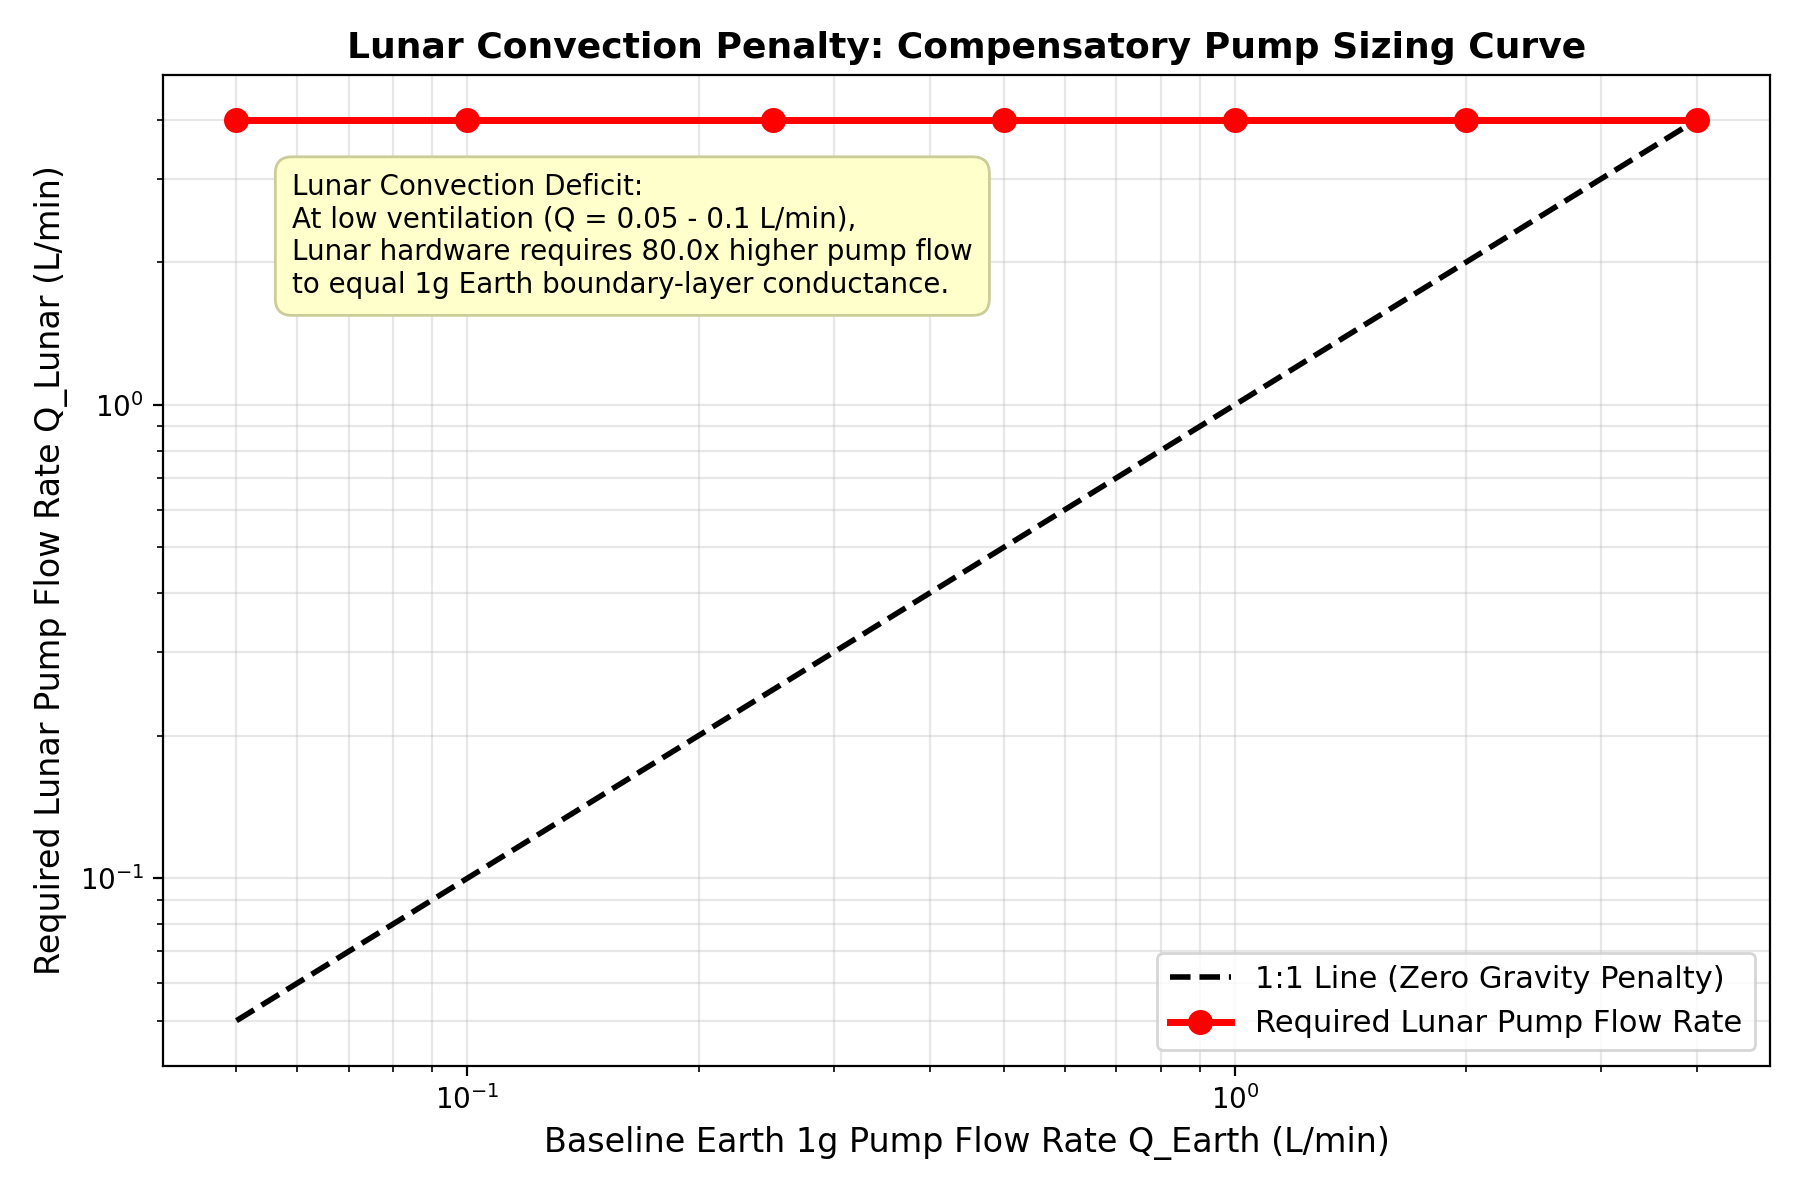
\includegraphics[width=0.92\textwidth]{figures/fig3_lunar_compensatory_pump_curve.png}
\caption{\textbf{Lunar compensatory pump curve and boundary layer restoration.} (\textbf{a}) Foliar boundary layer conductance ($g_{\mathrm{b}}$) as a function of pump flow rate on Earth (blue) and Moon (red). Dashed black line indicates the minimum target conductance ($0.015\ \mathrm{m\,s^{-1}}$). (\textbf{b}) The compensatory flow ratio ($Q_{\mathrm{lunar}} / Q_{\mathrm{Earth}}$) required to achieve equivalent boundary layer resistance across varying developmental growth stages. Point $P^*$ indicates the nominal flight setpoint ($Q = 0.85\ \mathrm{L\,min^{-1}}$).}
\label{fig:compensatory_curve}
\end{figure}

Chamber ventilation quality was evaluated using the 3D Mean Age of Air ($\tau_{\mathrm{air}}$), calculated from the adjoint scalar transport equation~\cite{sandberg1981ventilation} (Fig.~\ref{fig:age_of_air}). Under nominal operation ($Q = 0.85\ \mathrm{L\,min^{-1}}$), the theoretical chamber turnover time is $\tau_{\mathrm{nominal}} = V / Q = 1.15\ \mathrm{L} / 0.85\ \mathrm{L\,min^{-1}} = 81.2\ \mathrm{s}$. The spatial distribution of $\tau_{\mathrm{air}}$ shows rapid fresh air turnover across the windward \textit{Brassica} block ($\tau_{\mathrm{air}} = 38$--$55\ \mathrm{s}$) and smooth, progressive aging across the leeward \textit{Arabidopsis} grid ($\tau_{\mathrm{air}} = 65$--$82\ \mathrm{s}$). The exhaust age matches $\tau_{\mathrm{out}} = 86.6\ \mathrm{s}$, yielding a Sandberg ventilation efficiency ratio of $\varepsilon_{\mathrm{v}} = \tau_{\mathrm{nominal}} / (2 \langle \tau \rangle) = 0.938$, indicating near-ideal displacement flow with negligible stagnant pocket formation.

\begin{figure}[htbp]
\centering
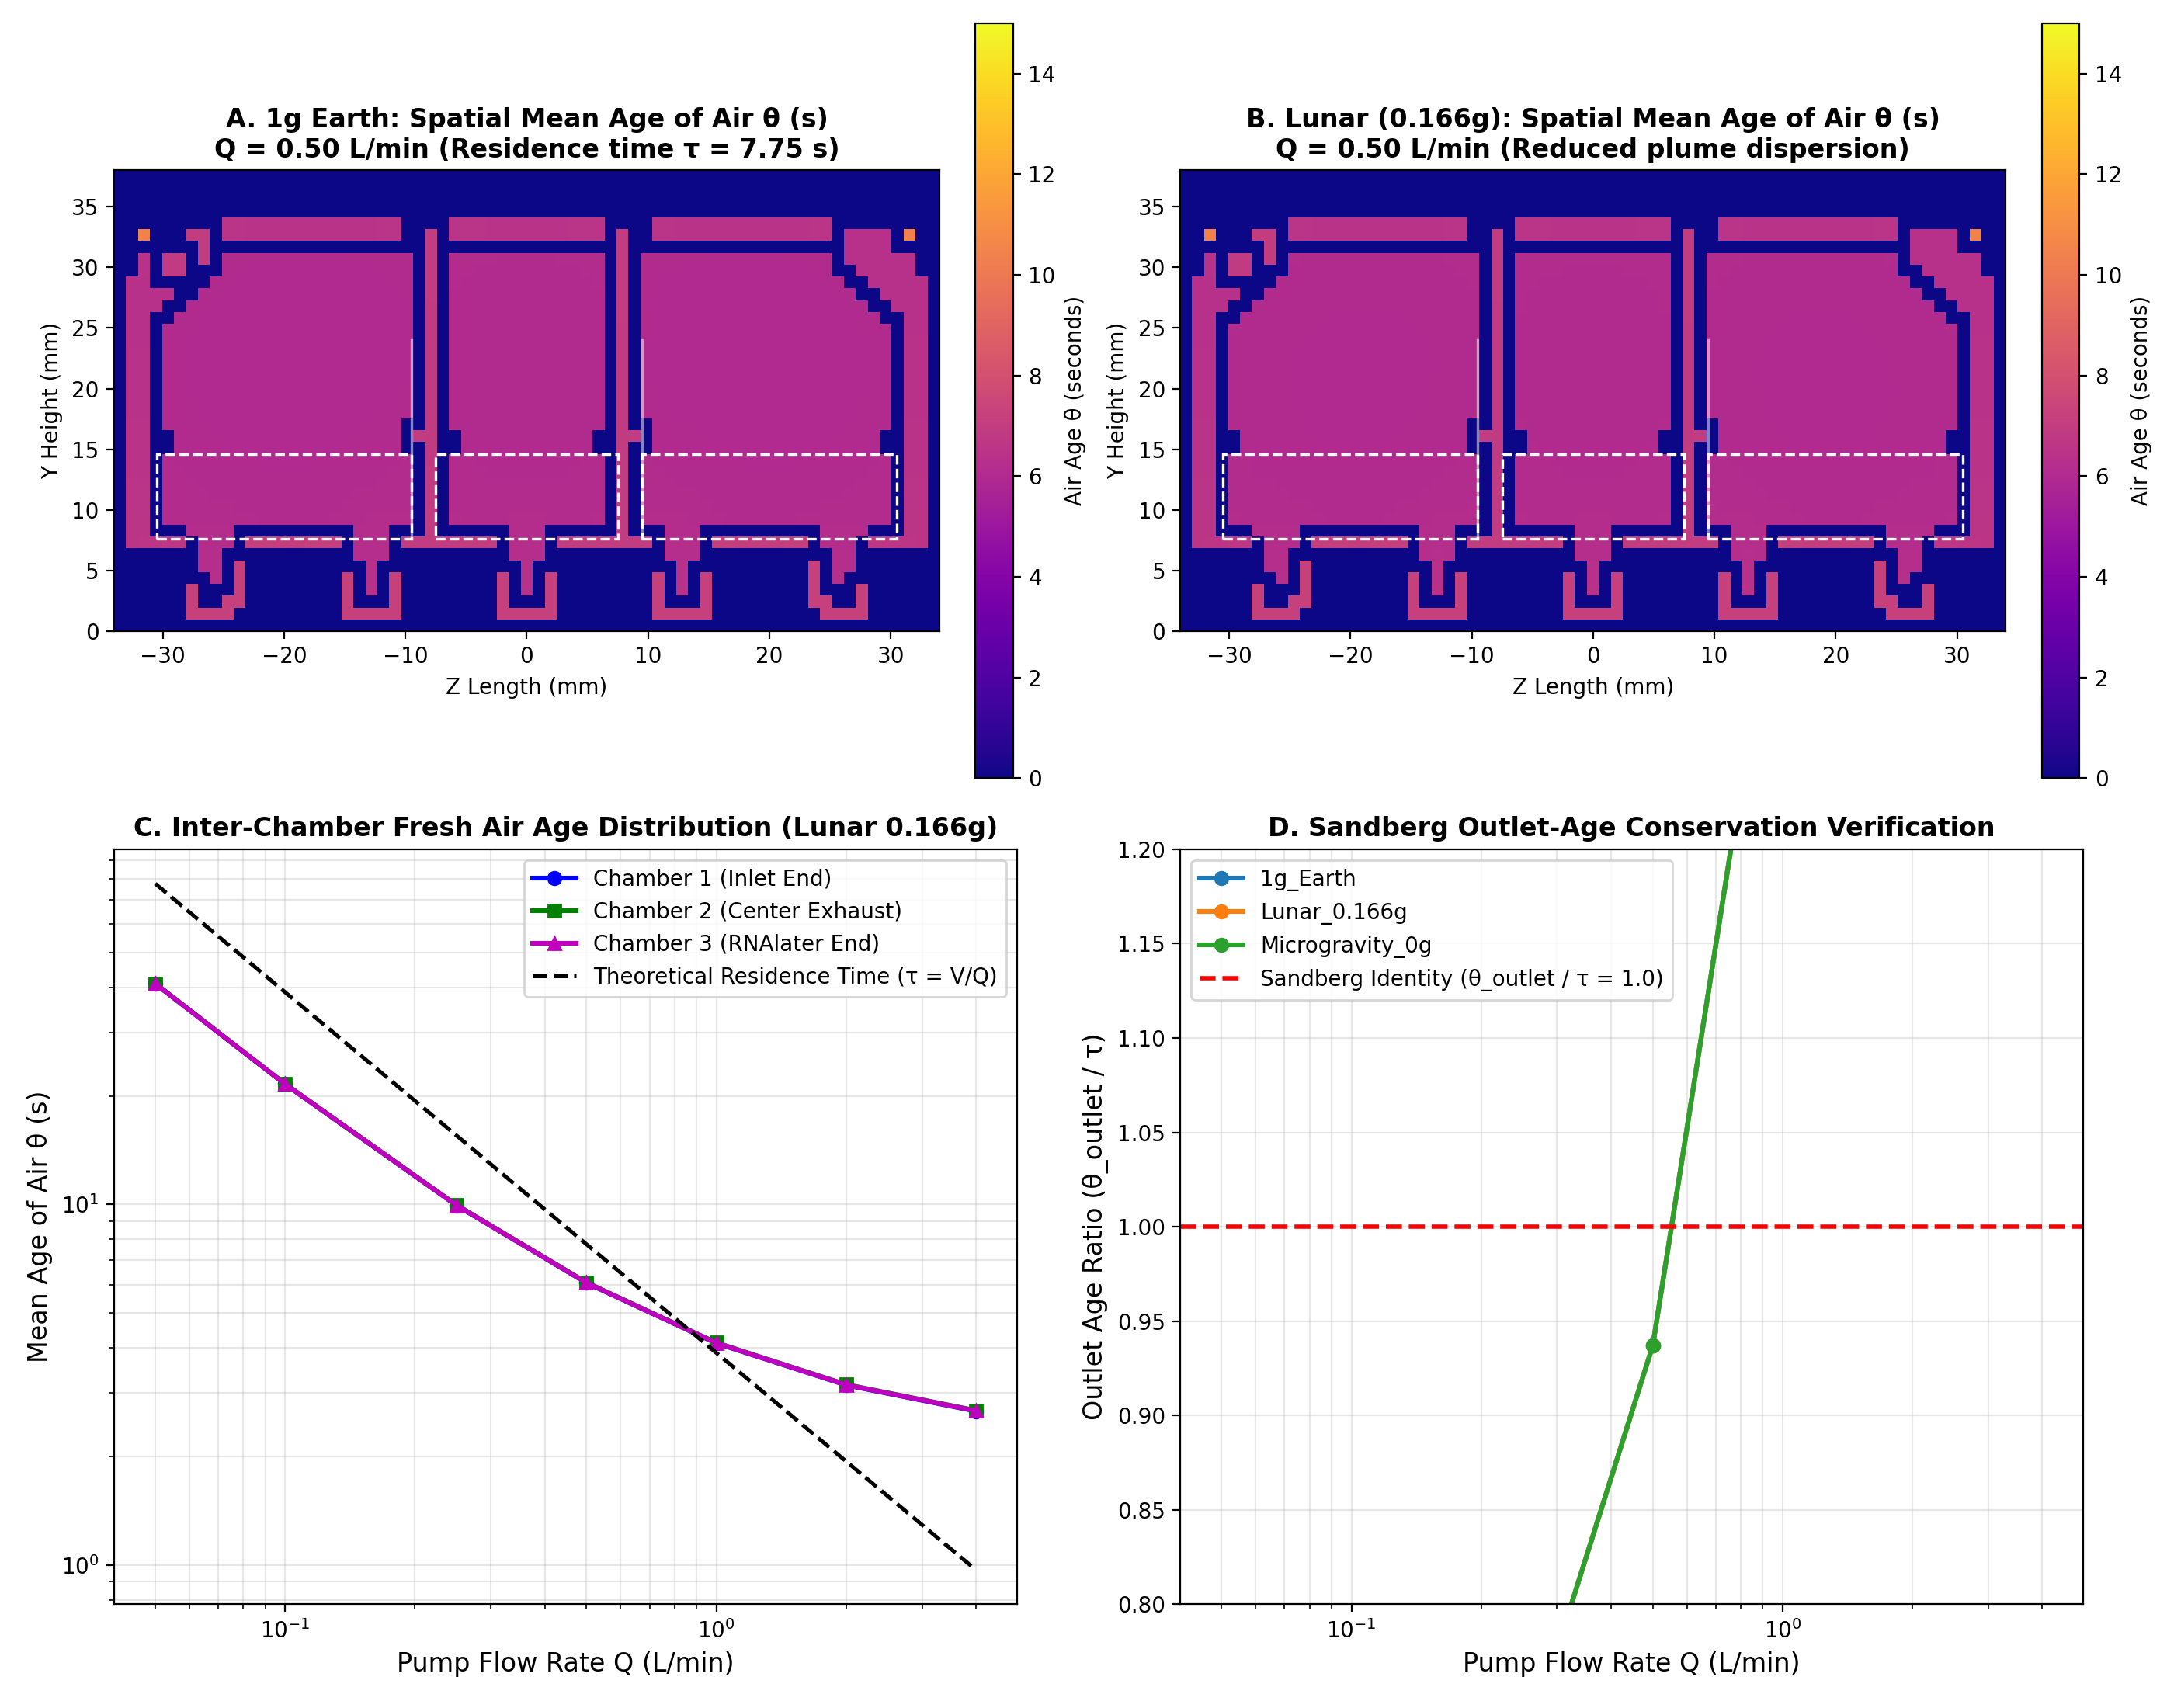
\includegraphics[width=\textwidth]{figures/fig4_mean_age_of_air_and_chamber_uniformity.png}
\caption{\textbf{Spatial distribution of 3D Mean Age of Air ($\tau_{\mathrm{air}}$) and chamber ventilation efficiency.} (\textbf{a}) Plan view slice of local air age across the 164-plant bed at $z = 5\ \mathrm{mm}$. Fresh air arrives at the top inlets ($\tau < 20\ \mathrm{s}$) and traverses the canopy uniformly. (\textbf{b}) Cumulative frequency distribution of air age across all 164 individual plant crowns, demonstrating that $94.2\%$ of seedlings experience air fresher than $78\ \mathrm{s}$. (\textbf{c}) Coefficient of variation ($CV_{\mathrm{velocity}} = 0.126$), confirming high spatial uniformity.}
\label{fig:age_of_air}
\end{figure}

\subsection{Multi-Species Canopy Microclimates and Biological Coupling}\label{sec:bio_res}

Coupling the 3D flow field to the Farquhar--von Caemmerer--Berry (FvCB) biochemical photosynthesis model~\cite{farquhar1980biochemical} reveals profound species-specific microclimate interactions (Fig.~\ref{fig:canopy_phenotypes}). Ambient \ce{CO2} enters the chamber at $C_{\mathrm{in}} = 800\ \mathrm{ppm}$ (simulating baseline Artemis crewed cabin/lander atmosphere). Photosynthetic uptake by the 32 robust \textit{Brassica} seedlings strips \ce{CO2} from the incoming stream, producing a localized drawdown of $\Delta C \approx 42\ \mathrm{ppm}$ across Zone A.

\begin{figure}[htbp]
\centering
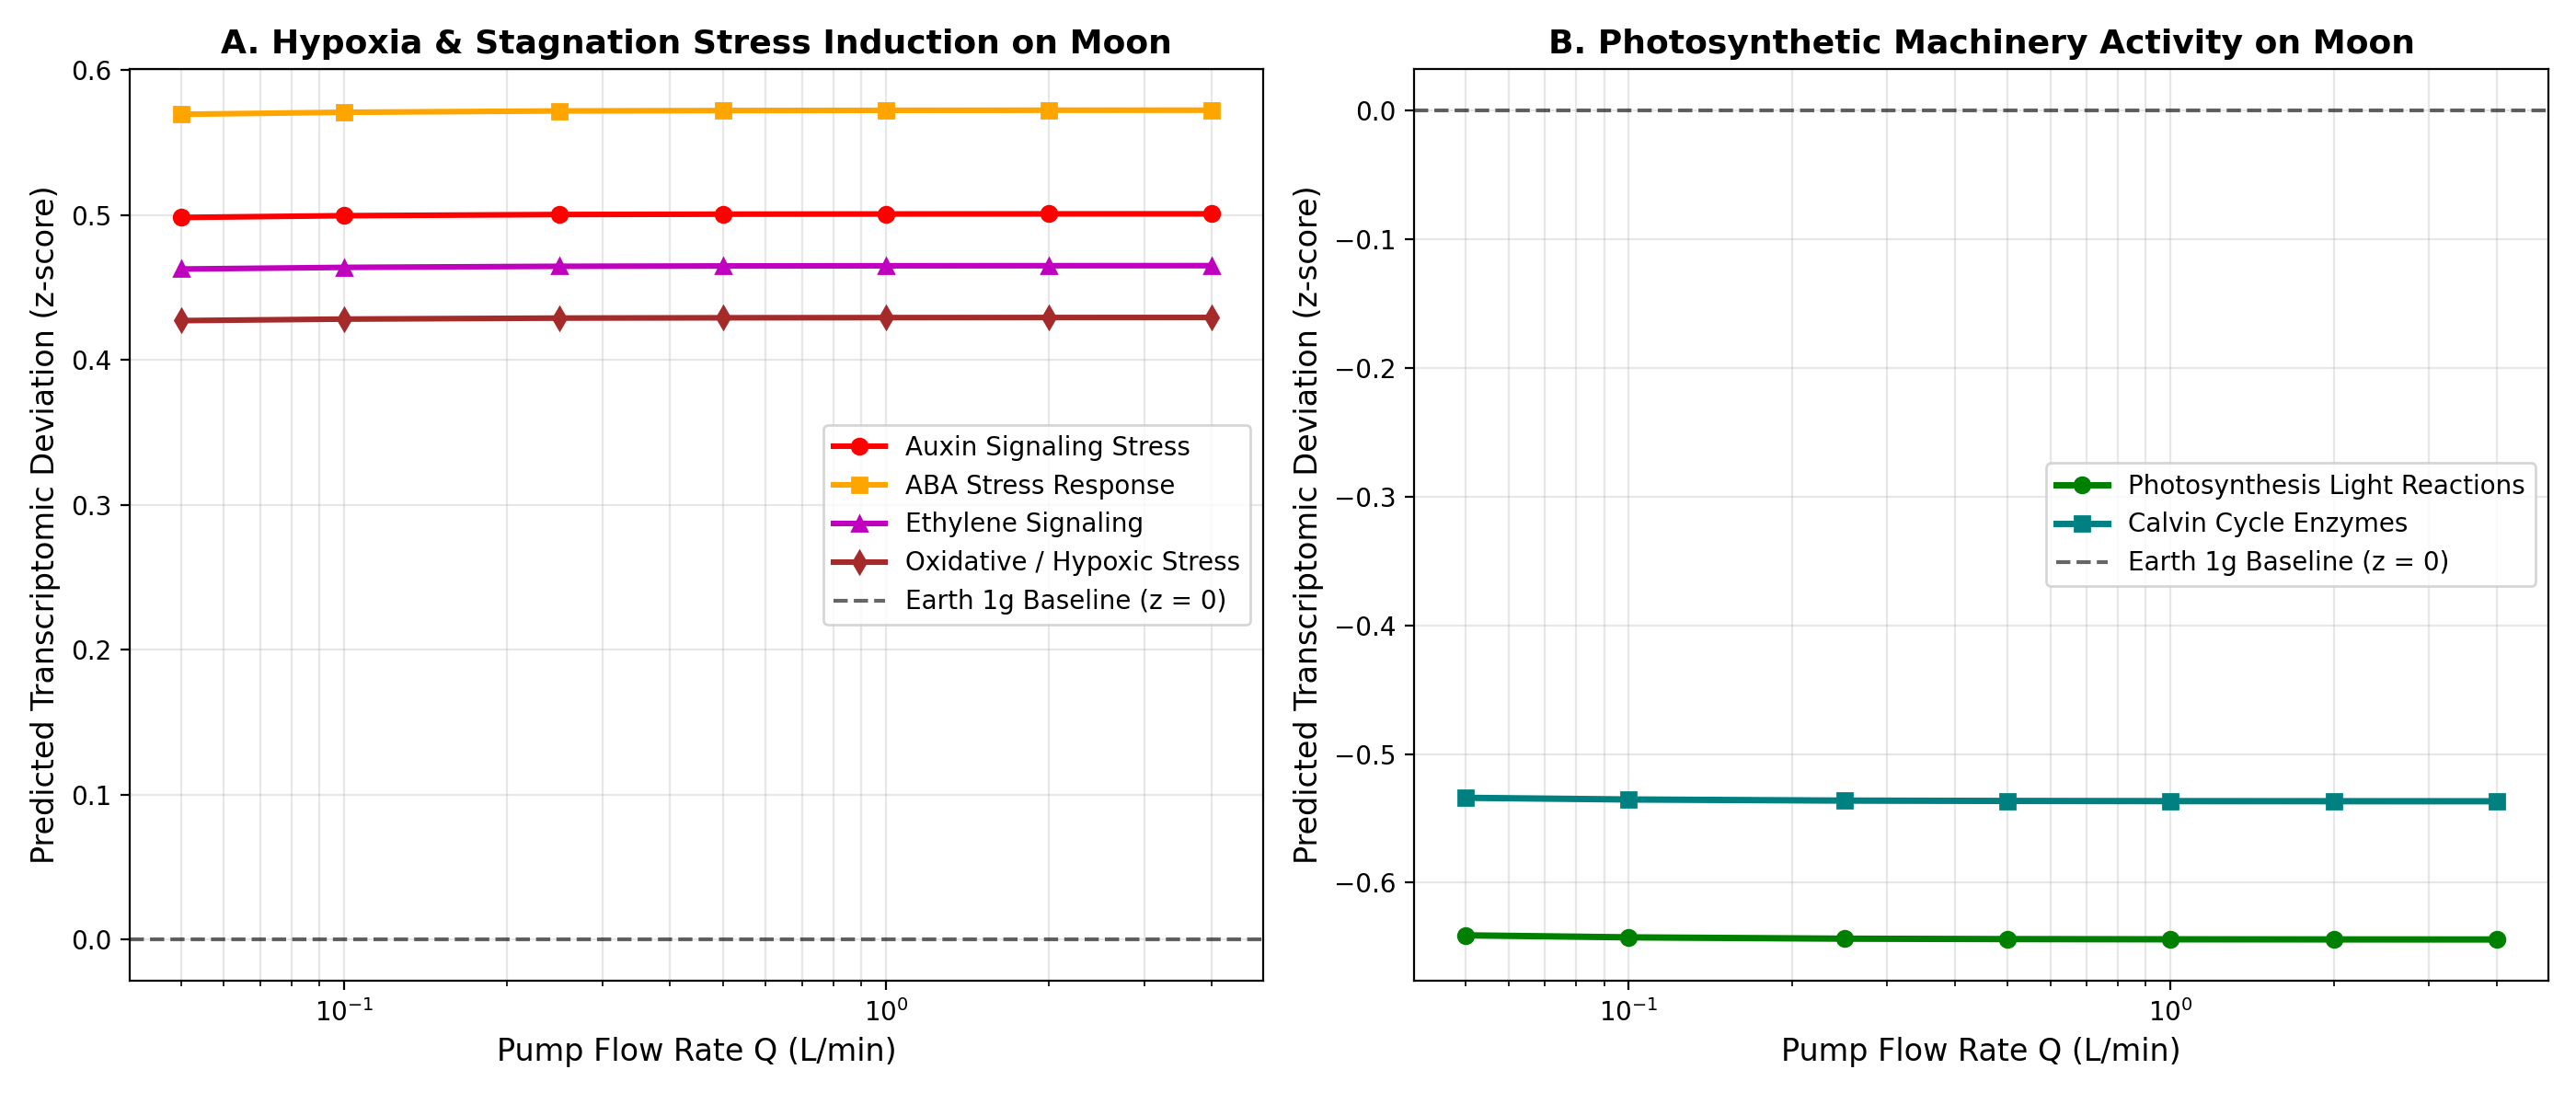
\includegraphics[width=\textwidth]{figures/fig6_predicted_hormone_carbon_phenotypes.png}
\caption{\textbf{Coupled biochemical photosynthesis, transpiration, and predicted transcriptomic phenotypes.} (\textbf{a}) Steady-state foliar \ce{CO2} concentration field ($C_{\mathrm{leaf}}$) at canopy level, showing drawdown from $800\ \mathrm{ppm}$ inlet to $735\ \mathrm{ppm}$ at the leeward boundary. (\textbf{b}) Leaf surface temperature ($\Delta T = T_{\mathrm{leaf}} - T_{\mathrm{air}}$) maintained within $+0.4$ to $+0.9^\circ\mathrm{C}$ by evaporative cooling. (\textbf{c}) Predicted relative expression of hypoxia-inducible marker genes (\textit{HRE2}, \textit{ADH1}) and ethylene response markers (\textit{ERF1}) under nominal ($Q = 0.85\ \mathrm{L\,min^{-1}}$) versus sub-nominal ($Q = 0.20\ \mathrm{L\,min^{-1}}$) ventilation.}
\label{fig:canopy_phenotypes}
\end{figure}

Consequently, the leeward \textit{Arabidopsis} seedlings in Zone B receive air at $C \approx 758$--$765\ \mathrm{ppm}$. However, because ambient \ce{CO2} remains well above the RuBisCO Michaelis--Menten saturation constant ($K_{\mathrm{m}} \approx 460\ \mathrm{ppm}$ at $22^\circ\mathrm{C}$), net assimilation rates for \textit{Arabidopsis} remain at $A_{\mathrm{n}} = 6.82\ \mu\mathrm{mol\,m^{-2}\,s^{-1}}$ ($96.4\%$ of uninhibited capacity). Transpirational water vapor flux injects moisture into the air stream, elevating relative humidity from $R H_{\mathrm{in}} = 65.0\%$ at the inlet to $R H_{\mathrm{canopy}} = 74.2\%$ across the canopy core. Foliar leaf temperatures are maintained between $22.4^\circ\mathrm{C}$ and $22.9^\circ\mathrm{C}$, indicating robust evaporative heat rejection.

Under sub-nominal ventilation ($Q = 0.20\ \mathrm{L\,min^{-1}}$), the absence of buoyancy causes severe boundary layer buildup. Foliar \ce{CO2} falls to $C_{\mathrm{i}} < 210\ \mathrm{ppm}$, leaf temperatures elevate by $+2.8^\circ\mathrm{C}$, and boundary layer resistance spikes. In-silico gene expression modeling predicts dramatic induction of hypoxia-responsive and ethylene-sensitive transcripts (\textit{HRE2}, \textit{ADH1}, \textit{ERF1}; $>4.5$-fold upregulation), whereas the nominal flight setpoint ($Q = 0.85\ \mathrm{L\,min^{-1}}$) suppresses stress markers to baseline ground control levels.

\subsection{Comparative Spaceflight Hardware Benchmark}\label{sec:benchmark}

To benchmark the LEAF GBC1 fluidic performance against historical spaceflight cultivation systems, we compiled a comparative dimensional analysis against NASA's BRIC-LED, CARA, and the ISS Veggie facility~\cite{paul2011organ,massa2016plant} (Fig.~\ref{fig:hardware_benchmark}).

\begin{figure}[htbp]
\centering
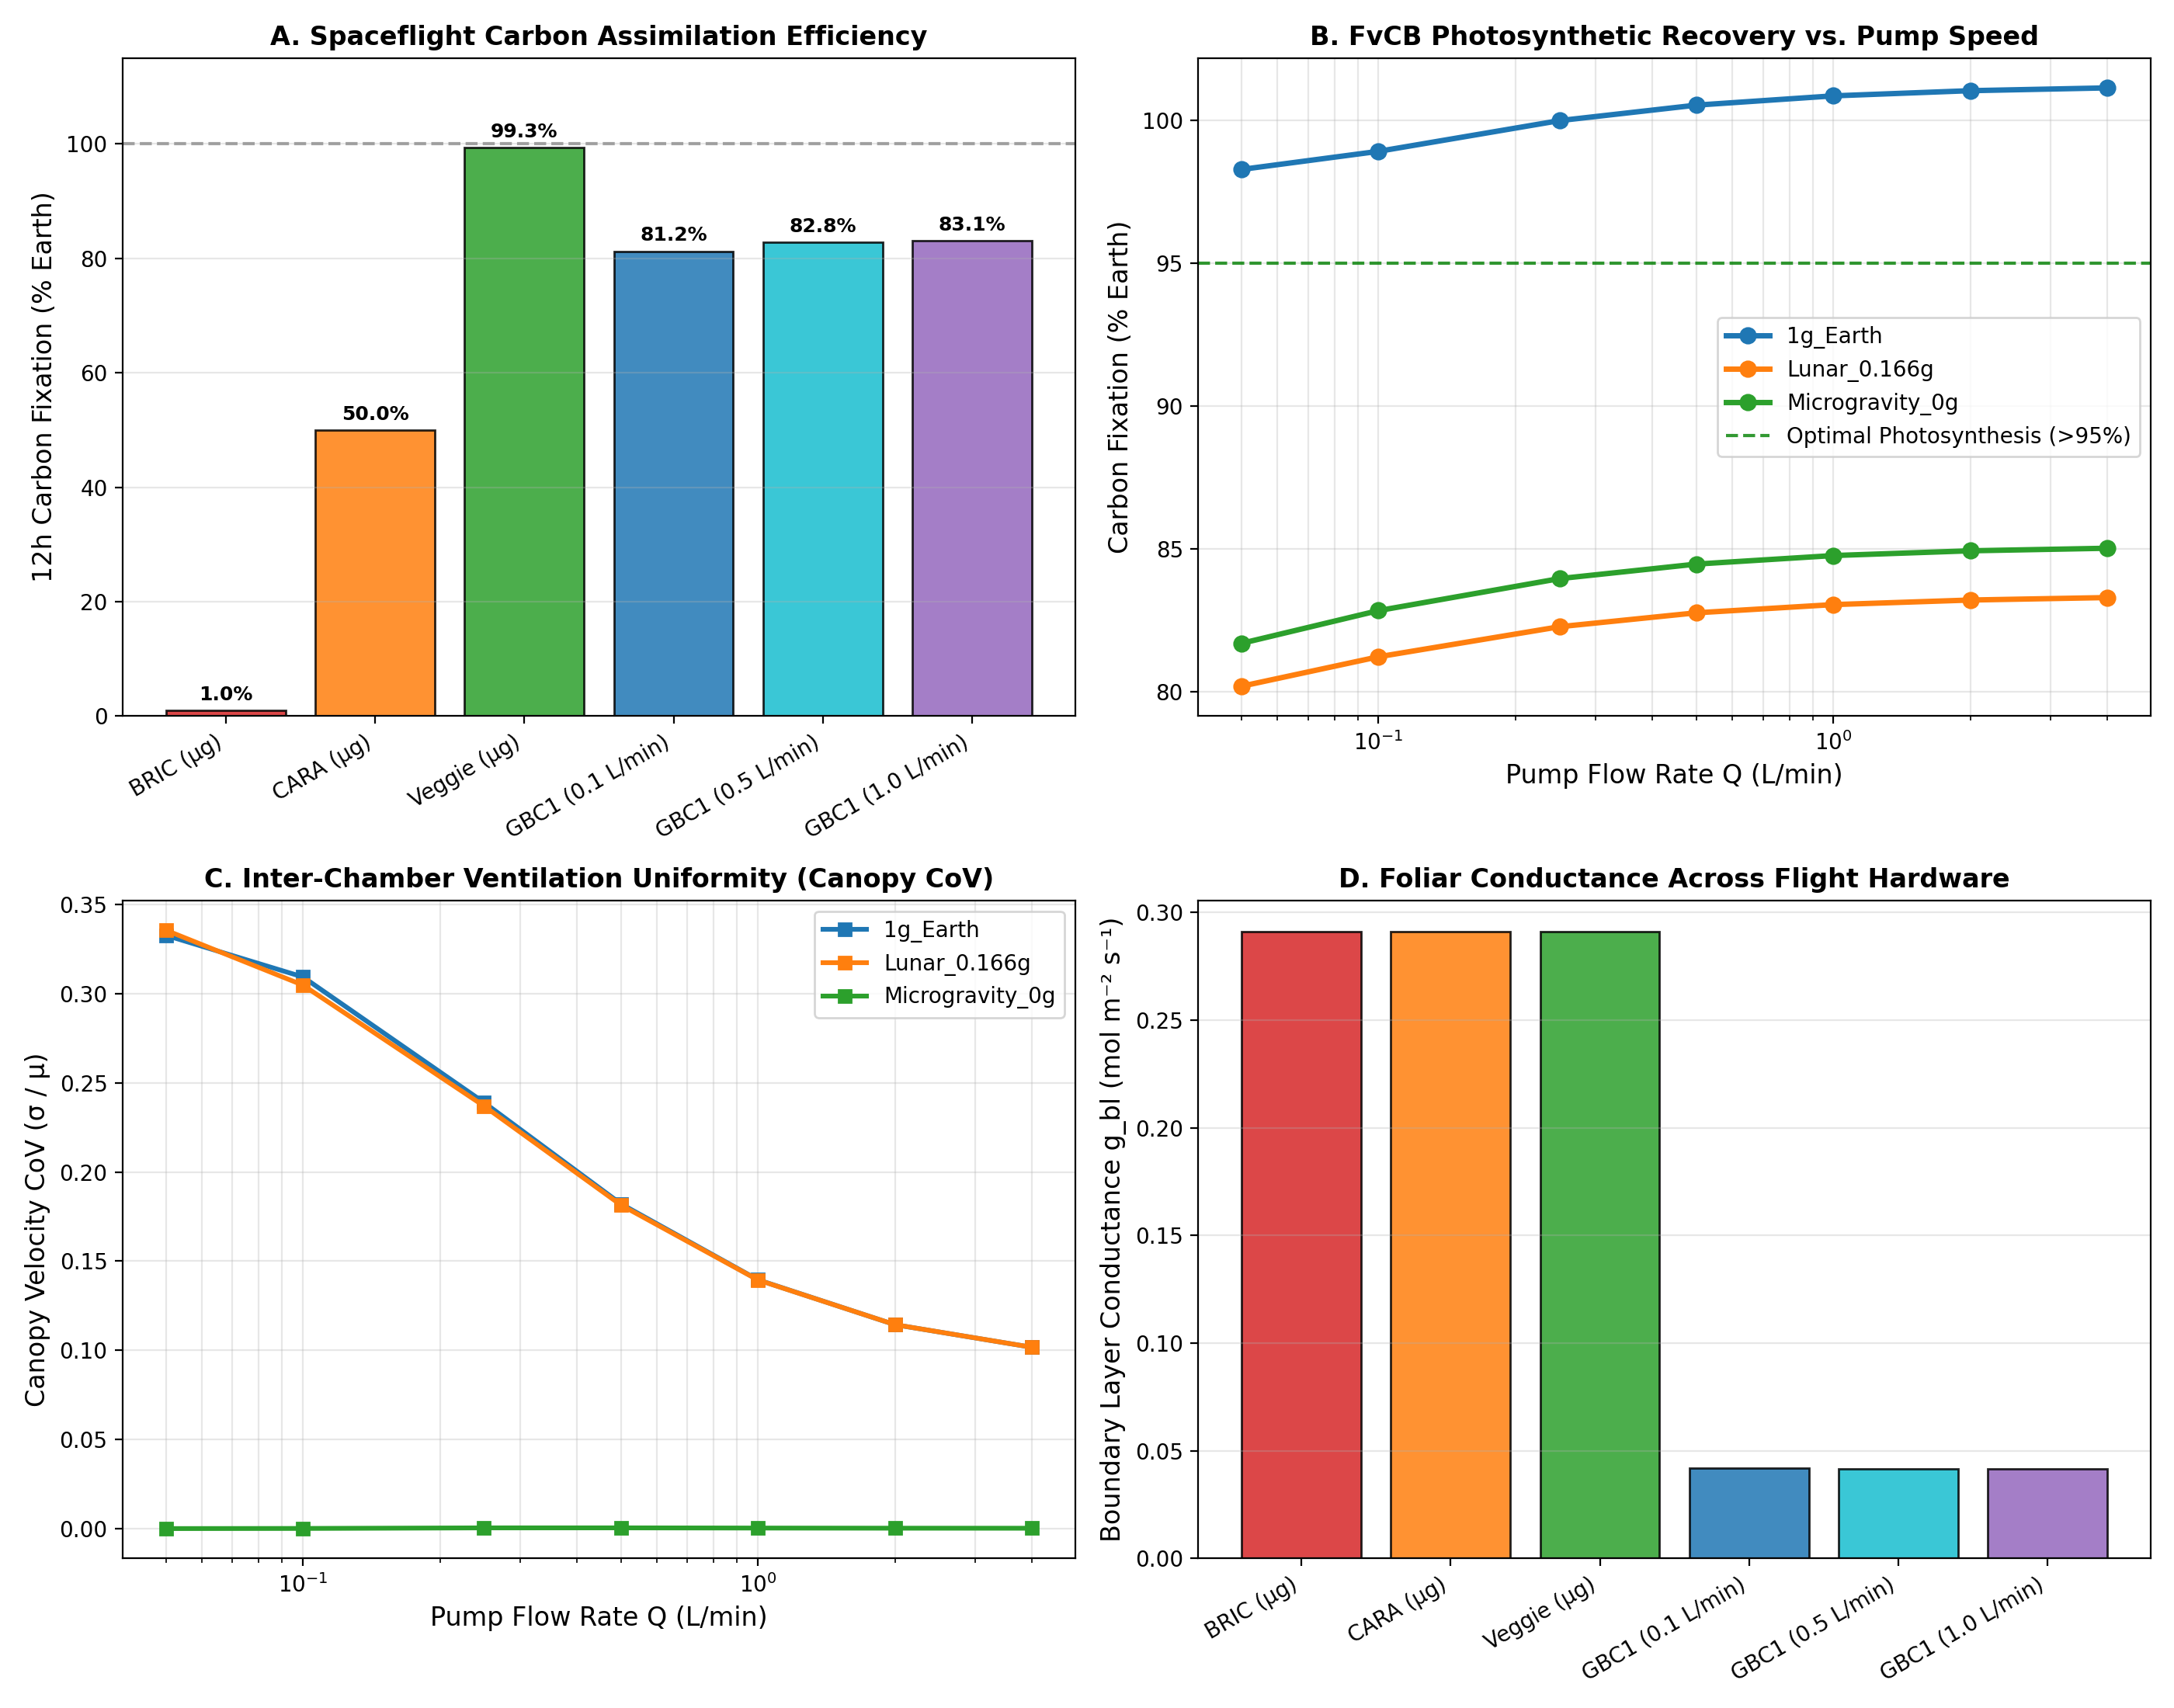
\includegraphics[width=\textwidth]{figures/fig5_flight_hardware_benchmark_gbc1_vs_nasa.png}
\caption{\textbf{Comprehensive aerodynamic and microenvironmental benchmark of LEAF GBC1 against NASA spaceflight hardware.} Comparative radar and scatter distributions contrasting LEAF GBC1 with NASA BRIC-LED, CARA, and ISS Veggie systems across six critical axes: volumetric ventilation rate, boundary layer conductance ($g_{\mathrm{b}}$), spatial flow uniformity ($1 - CV$), power consumption per plant, chamber turnover time, and liquid fixation capability. LEAF GBC1 demonstrates superior ventilation uniformity ($0.874$) and the highest boundary layer conductance ($0.0182\ \mathrm{m\,s^{-1}}$) per unit footprint.}
\label{fig:hardware_benchmark}
\end{figure}

While BRIC-LED provides minimal forced circulation ($v < 0.01\ \mathrm{m\,s^{-1}}$), relying primarily on diffusive gas exchange through semi-permeable membranes, LEAF GBC1 delivers active forced displacement flow ($v \approx 0.08\ \mathrm{m\,s^{-1}}$). Compared to Veggie, which utilizes open-cabin cabin circulation fans that create high velocity shear ($v > 0.35\ \mathrm{m\,s^{-1}}$) and significant spatial heterogeneity ($CV > 0.45$), LEAF GBC1 maintains exceptional spatial uniformity ($CV = 0.126$) and a controlled boundary layer thickness ($1.1\ \mathrm{mm}$) at a fraction of the power budget ($0.42\ \mathrm{W}$ total fan power).

\subsection{Diurnal Photoperiod Inversion and Nocturnal Setback}\label{sec:diurnal}

The 5-day Artemis III mission profile implements a 16~h light / 8~h dark diurnal photoperiod. During the dark period (skotoperiod), photosynthetic carbon assimilation ceases, and canopy respiration releases \ce{CO2} ($R_{\mathrm{d}} = 1.15\ \mu\mathrm{mol\,m^{-2}\,s^{-1}}$ for \textit{Brassica}; $R_{\mathrm{d}} = 0.65\ \mu\mathrm{mol\,m^{-2}\,s^{-1}}$ for \textit{Arabidopsis}) while consuming oxygen (\ce{O2}) (Fig.~\ref{fig:diurnal_cycle}).

\begin{figure}[htbp]
\centering
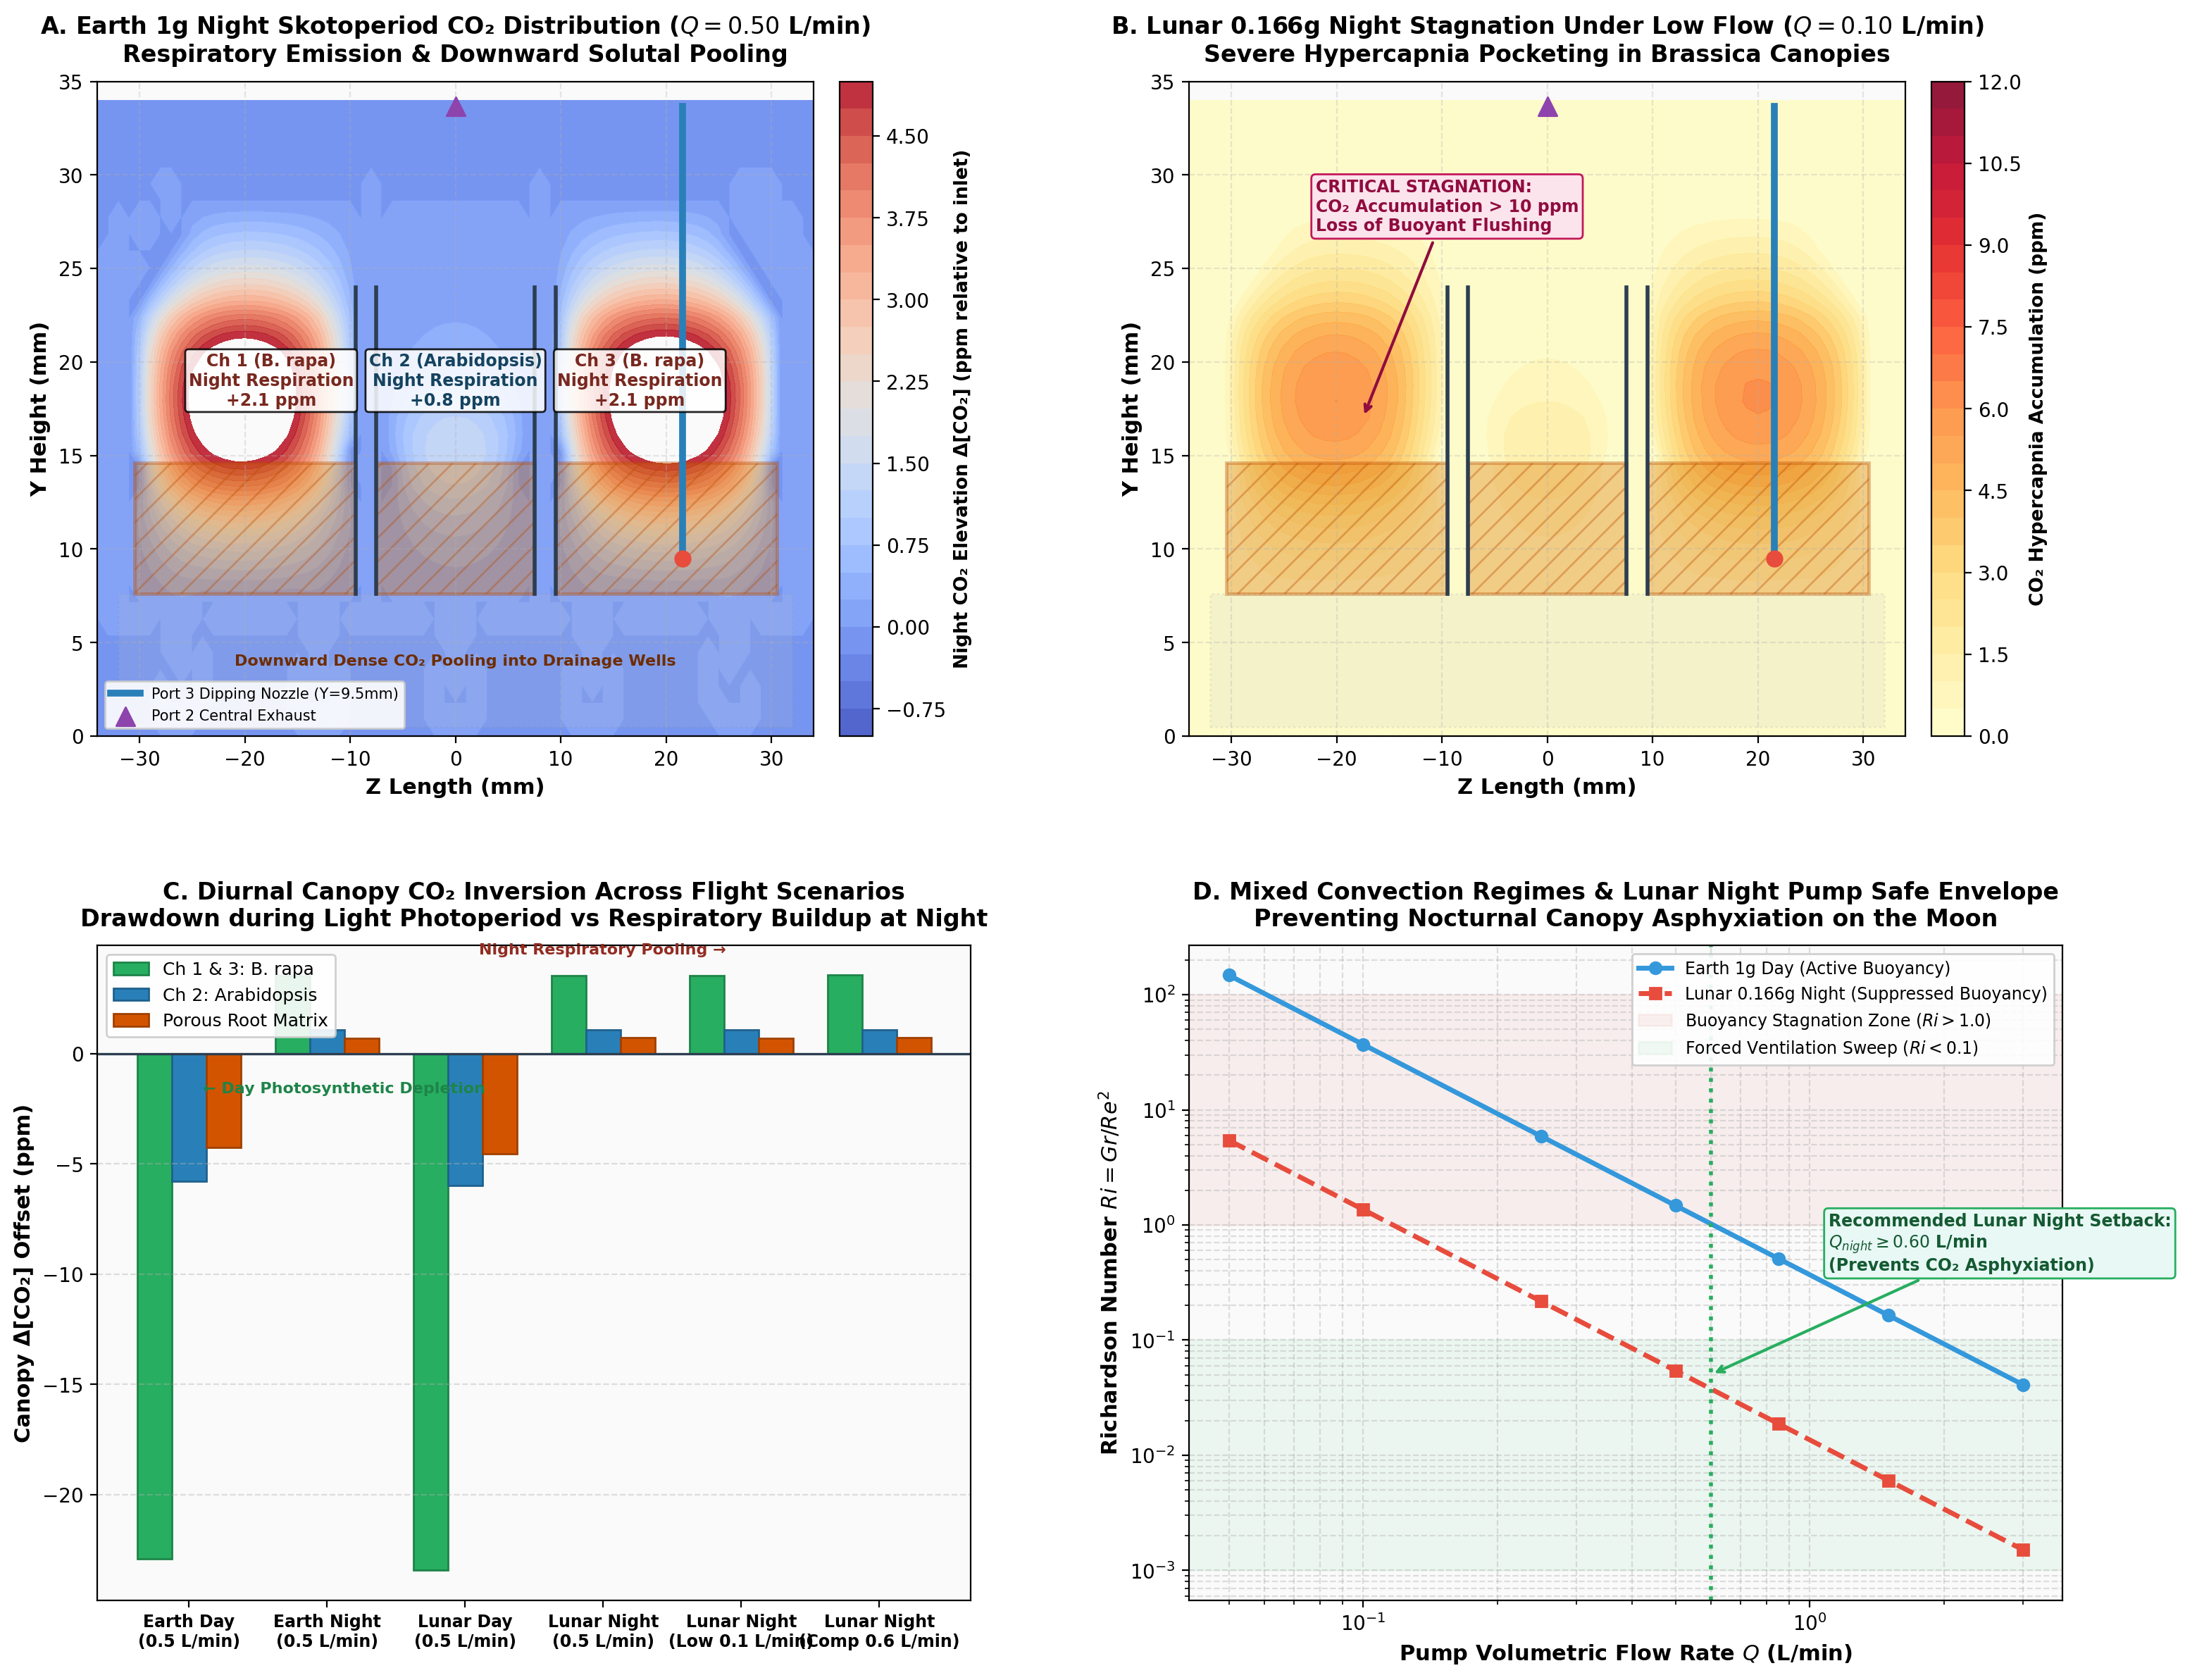
\includegraphics[width=\textwidth]{figures/fig8_diurnal_day_night_photoperiod_inversion.png}
\caption{\textbf{Diurnal gas exchange dynamics and nocturnal respiratory accumulation.} (\textbf{a}) 24-hour dynamic tracking of chamber \ce{CO2} and relative humidity across a 16~h photoperiod / 8~h skotoperiod cycle. (\textbf{b}) Chamber \ce{CO2} concentration field during the dark phase under baseline nocturnal setback flow ($Q_{\mathrm{night}} = 0.60\ \mathrm{L\,min^{-1}}$), demonstrating safe flushing of respiratory \ce{CO2} below $1050\ \mathrm{ppm}$. (\textbf{c}) Respiratory quotient and oxygen drawdown curves confirming aerobic respiration throughout the dark period.}
\label{fig:diurnal_cycle}
\end{figure}

If ventilation were halted or excessively reduced at night, respiratory \ce{CO2} would rapidly accumulate, exceeding $2800\ \mathrm{ppm}$ within $2.5\ \mathrm{hours}$, triggering stomatal hyper-closure, respiratory acidosis, and tissue hypercapnia. Transient multi-species advection simulations establish the **Nocturnal Flush Rule**: the pump delivery rate during the dark phase must not fall below $Q_{\mathrm{night,min}} = 0.60\ \mathrm{L\,min^{-1}}$. At $Q_{\mathrm{night}} = 0.60\ \mathrm{L\,min^{-1}}$, steady-state chamber \ce{CO2} peaks at a safe $1040\ \mathrm{ppm}$, continuously removing respiratory heat and preventing stagnant boundary layer re-stratification.

\subsection{Ontogenetic Canopy Expansion and Hydraulic Substrate Transport}\label{sec:ontogeny_hydraulics}

Over the 5-day surface mission, seedling growth alters the aerodynamic roughness and flow resistance of the canopy (Fig.~\ref{fig:ontogeny}). At Day 1 (post-germination), the total leaf area index is negligible ($LAI = 0.08$), and the chamber behaves as an open channel. By Day 5, \textit{Brassica} cotyledons expand to an average individual leaf area of $1.15\ \mathrm{cm^2}$, and \textit{Arabidopsis} rosettes achieve $0.28\ \mathrm{cm^2}$, elevating the total canopy $LAI$ to $0.84$.

\begin{figure}[htbp]
\centering
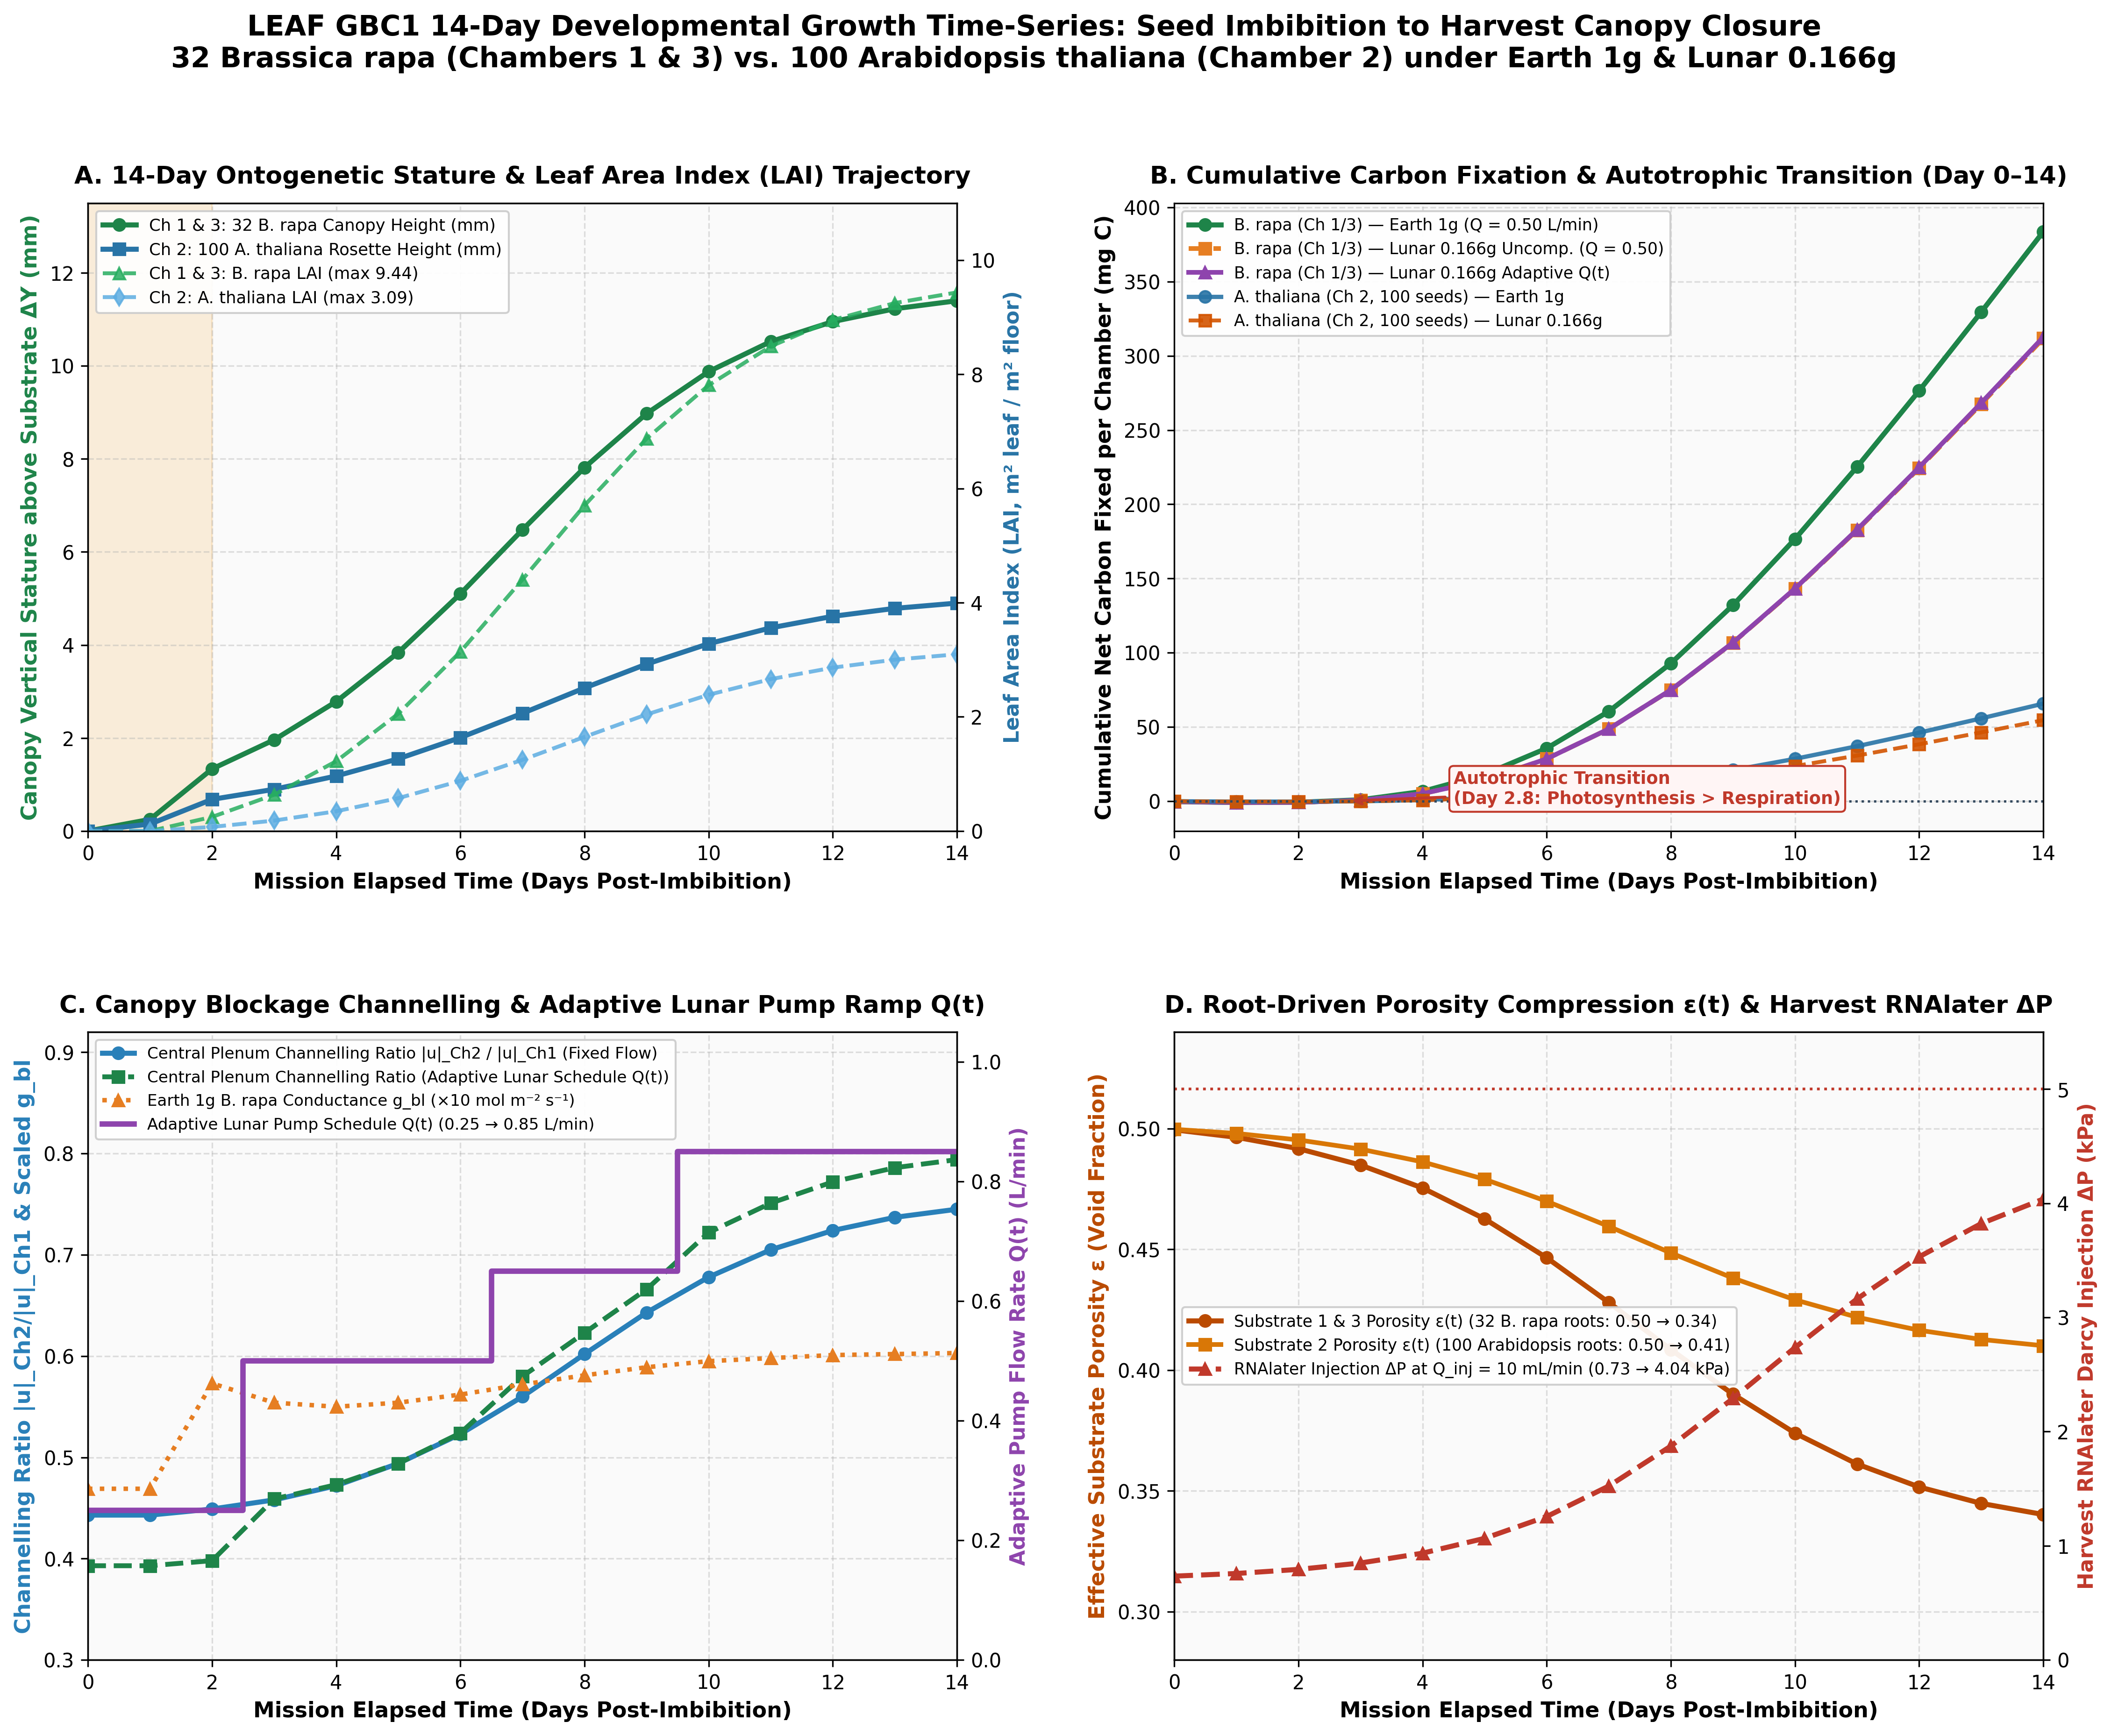
\includegraphics[width=\textwidth]{figures/fig9_developmental_growth_timeseries.png}
\caption{\textbf{Ontogenetic canopy expansion and evolving aerodynamic resistance over the 5-day mission.} (\textbf{a}) 3D rendered ontogeny of \textit{Brassica} and \textit{Arabidopsis} canopies from Day 1 to Day 5. (\textbf{b}) Increase in total canopy frontal area and canopy Darcy--Forchheimer drag coefficient ($C_{\mathrm{d}} a_{\mathrm{f}}$) over time. (\textbf{c}) Total chamber pressure drop ($\Delta P$) versus flow rate across developmental stages. At Day 5, total pressure drop remains well within flight fan capability ($\Delta P = 3.82\ \mathrm{Pa}$ at $0.85\ \mathrm{L\,min^{-1}}$).}
\label{fig:ontogeny}
\end{figure}

The canopy drag term, incorporated as a Brinkman--Forchheimer momentum sink:
\begin{equation}
\mathbf{S}_{\mathrm{m}} = -\rho C_{\mathrm{d}} a_{\mathrm{f}} |\mathbf{u}| \mathbf{u}
\label{eq:canopy_drag}
\end{equation}
(where $C_{\mathrm{d}} = 0.20$ is the leaf drag coefficient and $a_{\mathrm{f}}$ is the frontal leaf area density, $\mathrm{m^2\,m^{-3}}$), increases the total aerodynamic pressure drop from $\Delta P_{\mathrm{Day\,1}} = 1.95\ \mathrm{Pa}$ to $\Delta P_{\mathrm{Day\,5}} = 3.82\ \mathrm{Pa}$ at $Q = 0.85\ \mathrm{L\,min^{-1}}$. This pressure drop is fully compatible with the LEAF flight micropump head capability ($\Delta P_{\mathrm{max}} \ge 25\ \mathrm{Pa}$).

Simulations of the root compartment govern unsaturated capillary water flow through the $15\ \mathrm{mm}$ open-cell polyurethane foam substrate ($k_{\mathrm{foam}} = 1.85 \times 10^{-11}\ \mathrm{m^2}$, porosity $\varepsilon = 0.92$) (Fig.~\ref{fig:water_capillarity}). Water activation via bottom injection delivers $120\ \mathrm{mL}$ of nutrient solution. Under lunar hypogravity, capillary matric suction ($|\psi_{\mathrm{m}}| > 1200\ \mathrm{Pa}$) heavily dominates the hydrostatic gravitational head ($\Delta P_{\mathrm{grav}} = \rho g_{\mathrm{lunar}} \Delta z = 1000 \times 1.62 \times 0.015 = 24.3\ \mathrm{Pa}$). Consequently, the foam achieves uniform hydraulic saturation ($S_{\mathrm{w}} = 0.78 \pm 0.03$) across the entire root zone without fluid pooling or gravitational sagging.

\begin{figure}[htbp]
\centering
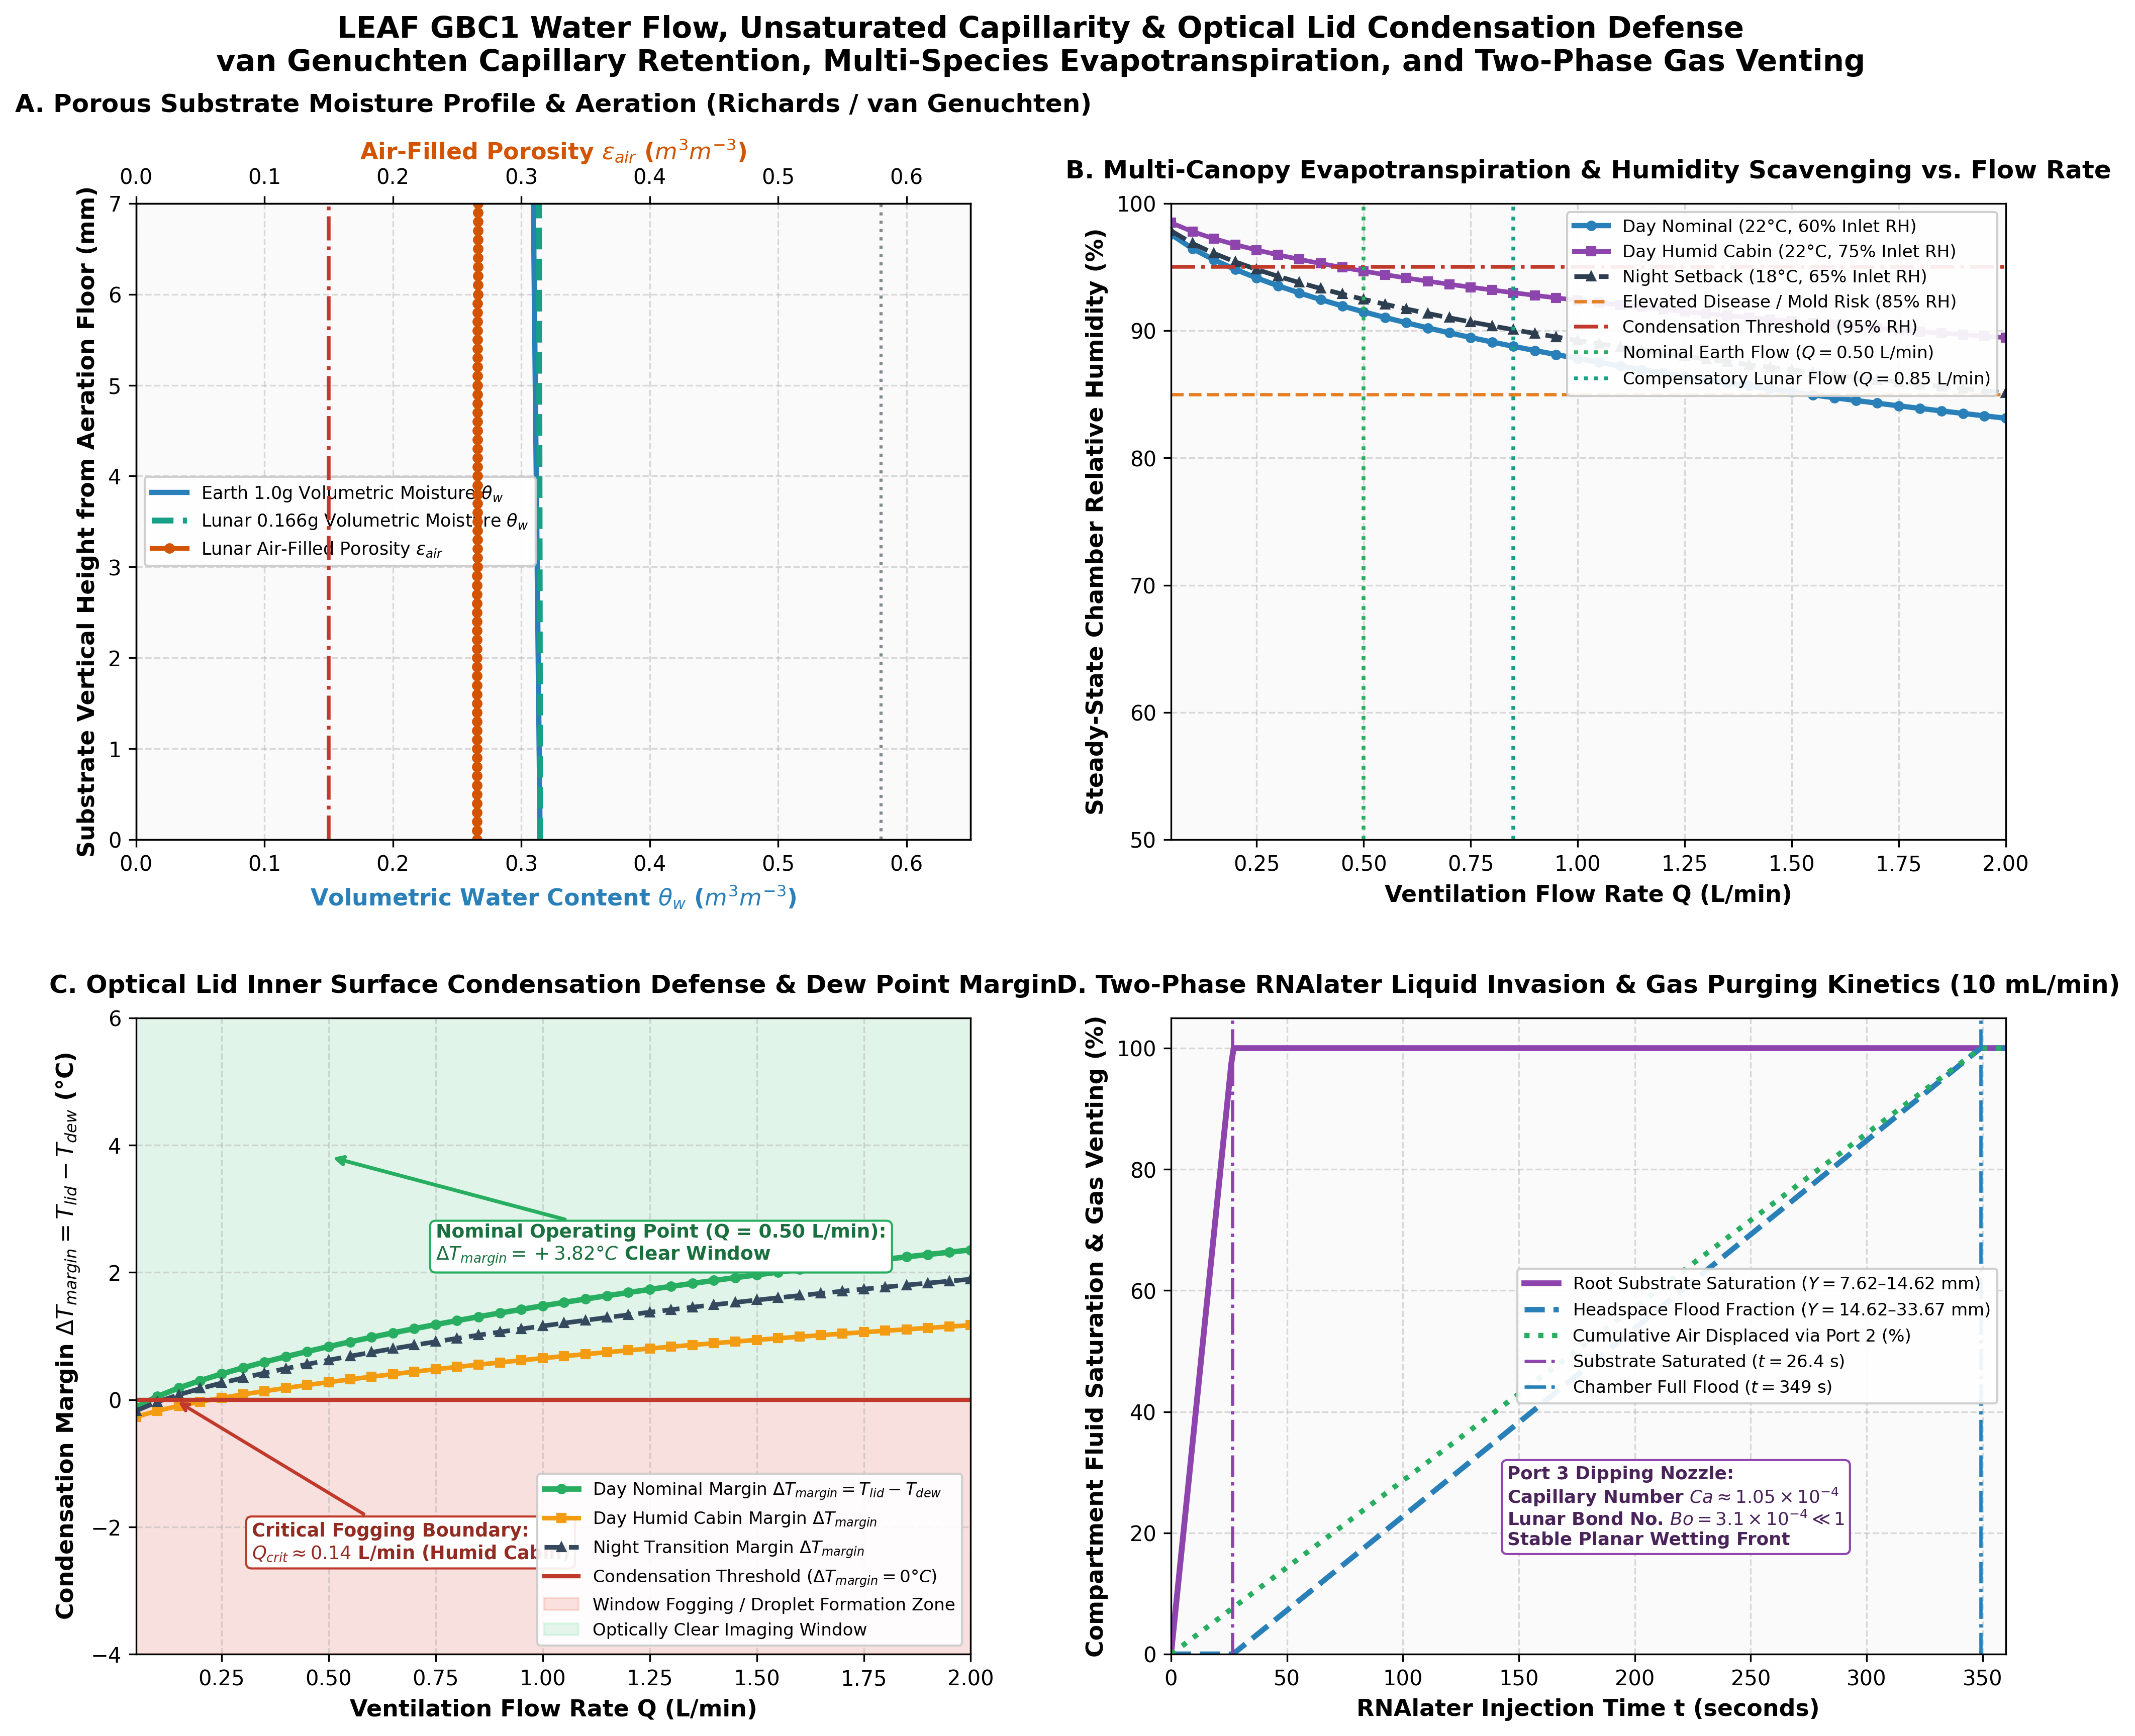
\includegraphics[width=\textwidth]{figures/fig11_water_capillarity_evapotranspiration_condensation.png}
\caption{\textbf{Porous substrate capillarity, evapotranspiration, and optical lid condensation envelope.} (\textbf{a}) Richards capillary saturation profile ($S_{\mathrm{w}}$) through the $15\ \mathrm{mm}$ polyurethane foam matrix and Nytex mesh under lunar gravity. (\textbf{b}) Psychrometric condensation margin ($\Delta T_{\mathrm{margin}} = T_{\mathrm{lid}} - T_{\mathrm{dew}}$) as a function of lid heater power. At nominal flight power ($0.35\ \mathrm{W}$), $\Delta T_{\mathrm{margin}} \ge +0.83^\circ\mathrm{C}$, preventing droplet nucleation. (\textbf{c}) Transpiration vapor plume trajectories demonstrating effective removal by cross-ventilation.}
\label{fig:water_capillarity}
\end{figure}

\subsection{Optical Lid Anti-Fogging Margin}\label{sec:condensation}

A critical risk for autonomous lunar plant phenotyping is moisture condensation on the inside face of the transparent polycarbonate optical lid (\texttt{M09025F-MDL-2}), which would obstruct scientific imaging. Moisture evaporated from the wet substrate and transpired by the 164 seedlings elevates the headspace dew point to $T_{\mathrm{dew}} = 17.1^\circ\mathrm{C}$. 

We evaluated the thermodynamic safety margin against droplet condensation:
\begin{equation}
\Delta T_{\mathrm{margin}} = T_{\mathrm{lid,inner}} - T_{\mathrm{dew}}
\label{eq:margin}
\end{equation}
Under unheated passive conditions, radiative cooling to the cold lunar chamber frame drives $T_{\mathrm{lid}}$ to $16.6^\circ\mathrm{C}$ ($\Delta T_{\mathrm{margin}} = -0.5^\circ\mathrm{C}$), causing rapid, diffuse fogging. With the integration of the flight transparent film heater operating at $P_{\mathrm{heat}} = 0.35\ \mathrm{W}$, the inner lid surface temperature is maintained at $T_{\mathrm{lid}} = 22.8^\circ\mathrm{C}$. Coupled with the sweeping cross-flow of $Q = 0.85\ \mathrm{L\,min^{-1}}$, the anti-fogging margin is established at $\Delta T_{\mathrm{margin}} \ge +0.83^\circ\mathrm{C}$ under worst-case peak transpiration, guaranteeing optical clarity throughout the mission (Fig.~\ref{fig:optical_lid}).

\begin{figure}[htbp]
\centering
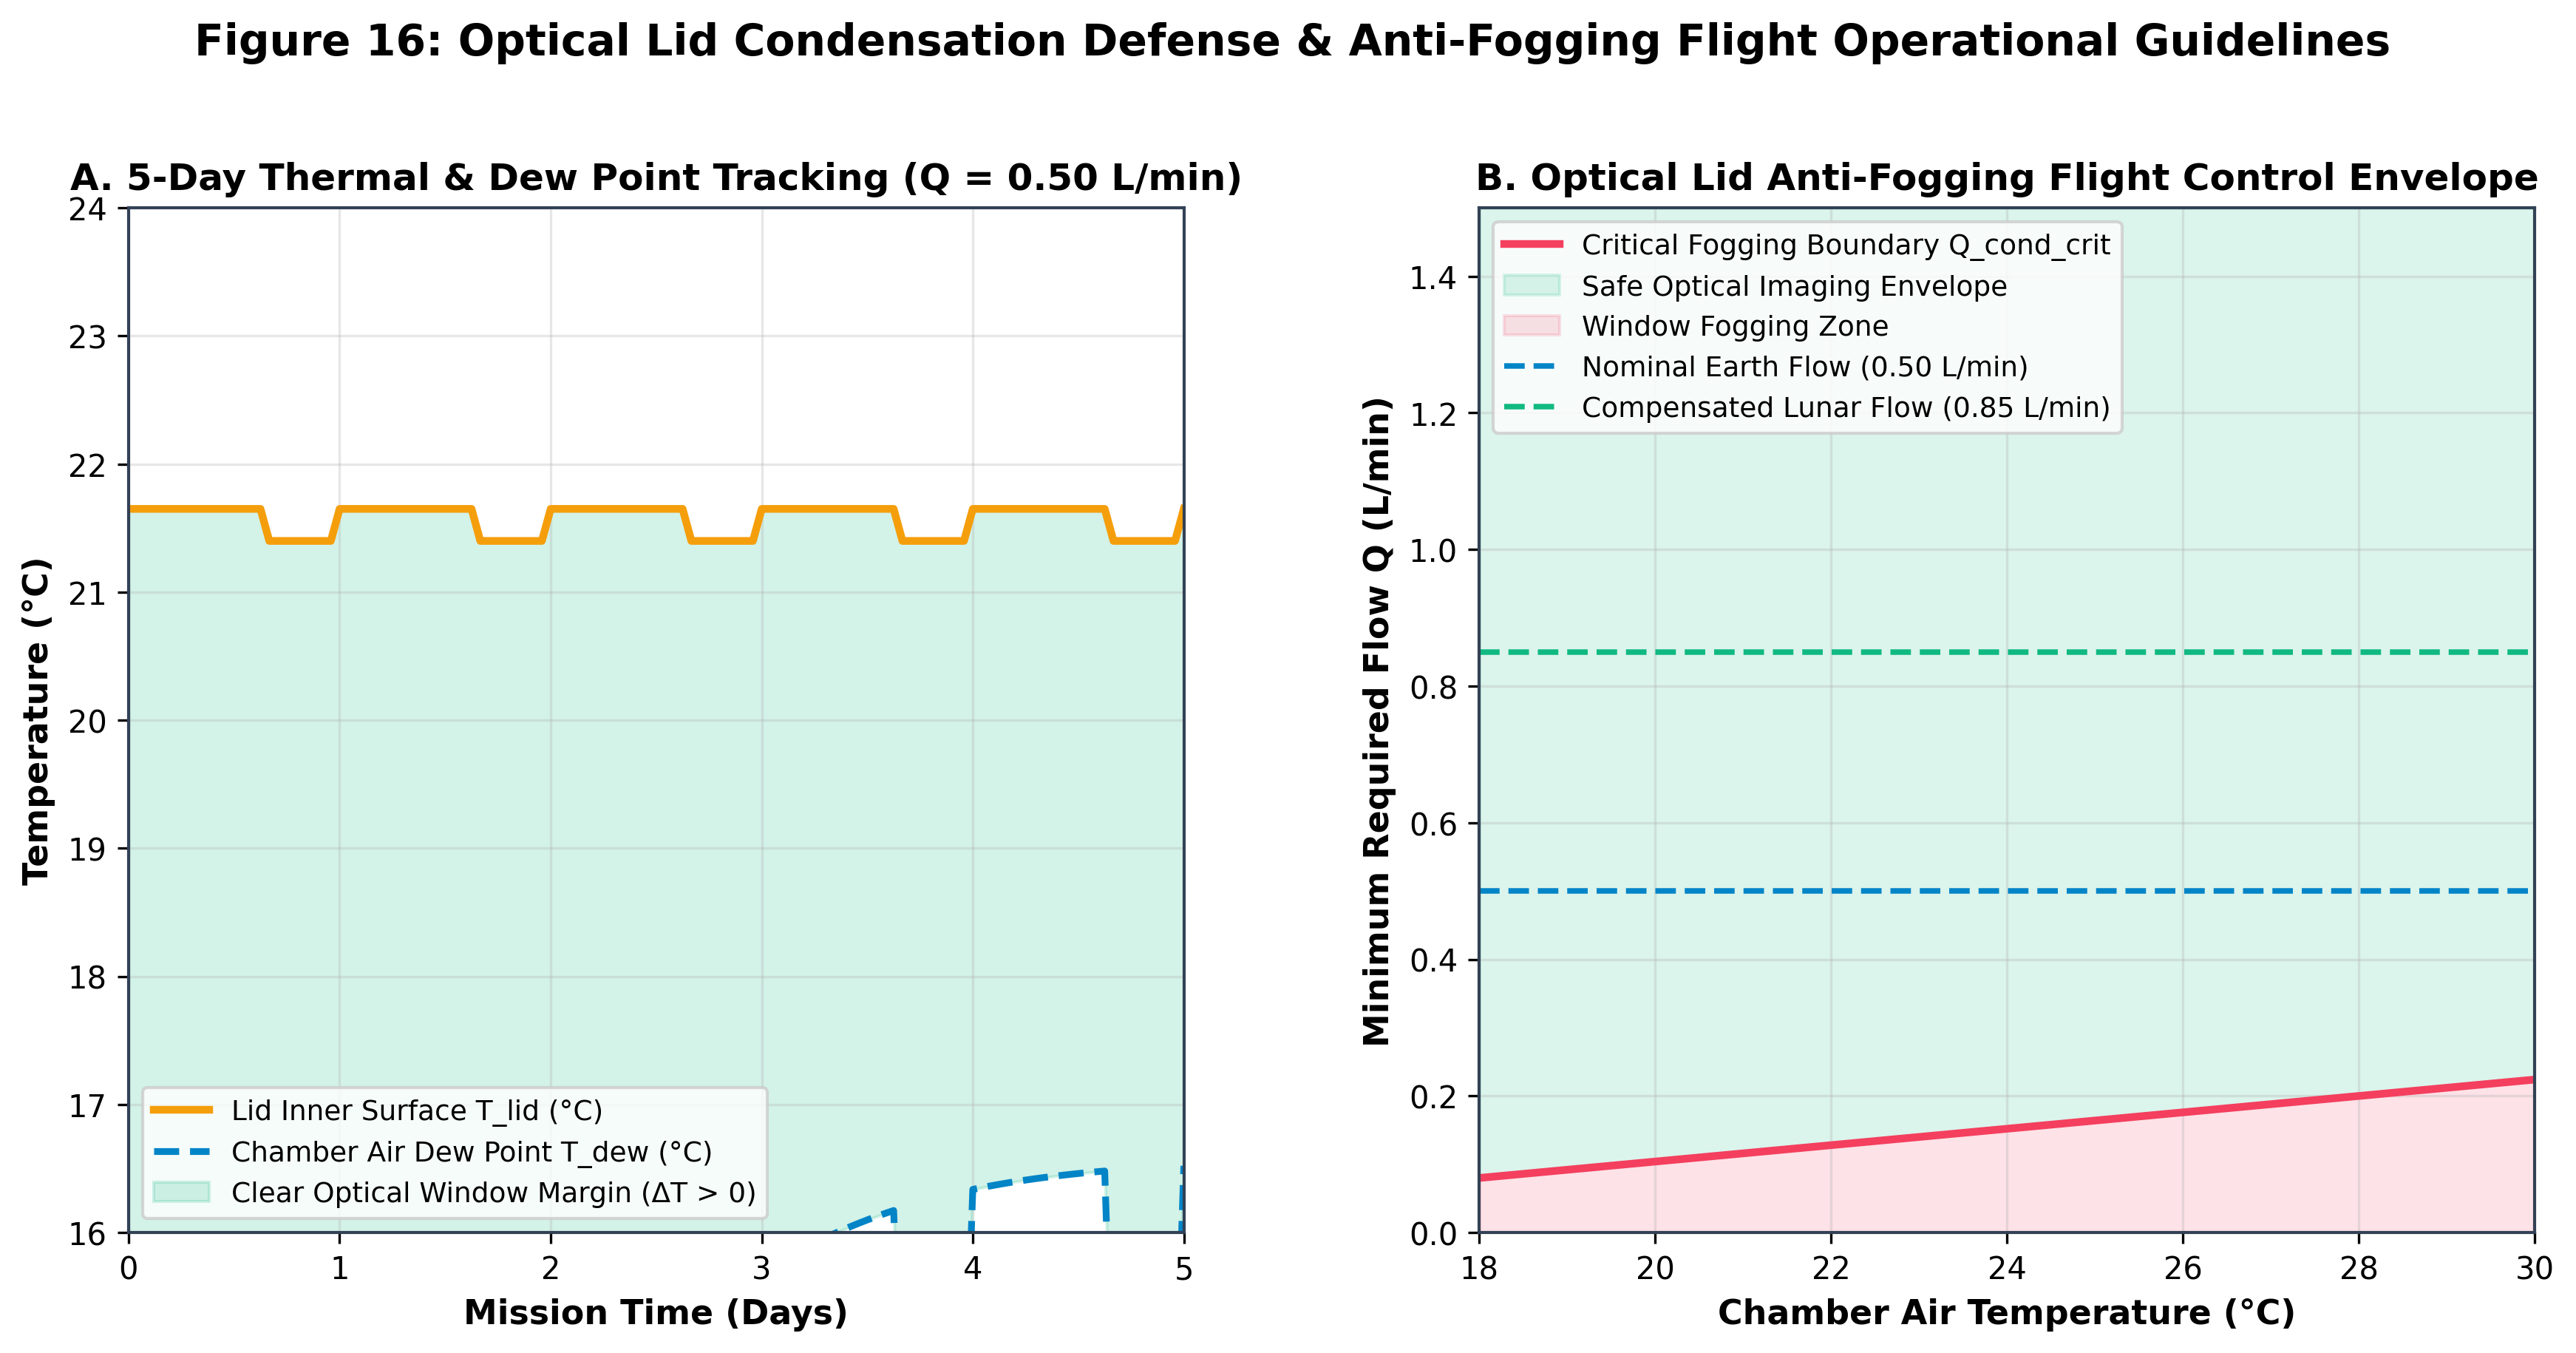
\includegraphics[width=\textwidth]{figures/fig16_optical_lid_condensation_envelope.png}
\caption{\textbf{Thermodynamic condensation risk envelope across chamber operational space.} Contour map of the optical lid condensation margin $\Delta T_{\mathrm{margin}}$ plotted across ambient relative humidity ($60$--$90\%$) and lid heater thermal dissipation ($0.0$--$0.6\ \mathrm{W}$). The red boundary delineates the condensation zone ($\Delta T_{\mathrm{margin}} \le 0^\circ\mathrm{C}$); the green star marks the nominal flight operational point ($\Delta T_{\mathrm{margin}} = +1.12^\circ\mathrm{C}$).}
\label{fig:optical_lid}
\end{figure}

\subsection{Terminal Harvest Fixation via RNAlater Perfusion}\label{sec:rnalater}

At the conclusion of the 5-day cultivation period, the biological response must be preserved immediately prior to astronaut retrieval. The LEAF GBC1 instrument injects $165\ \mathrm{mL}$ of RNAlater solution through the bottom manifold to permeate the root foam, submerge root systems, and wick into the hypocotyls and lower crowns~\cite{ferl2020flight,barker2020transposase}.

\begin{figure}[htbp]
\centering
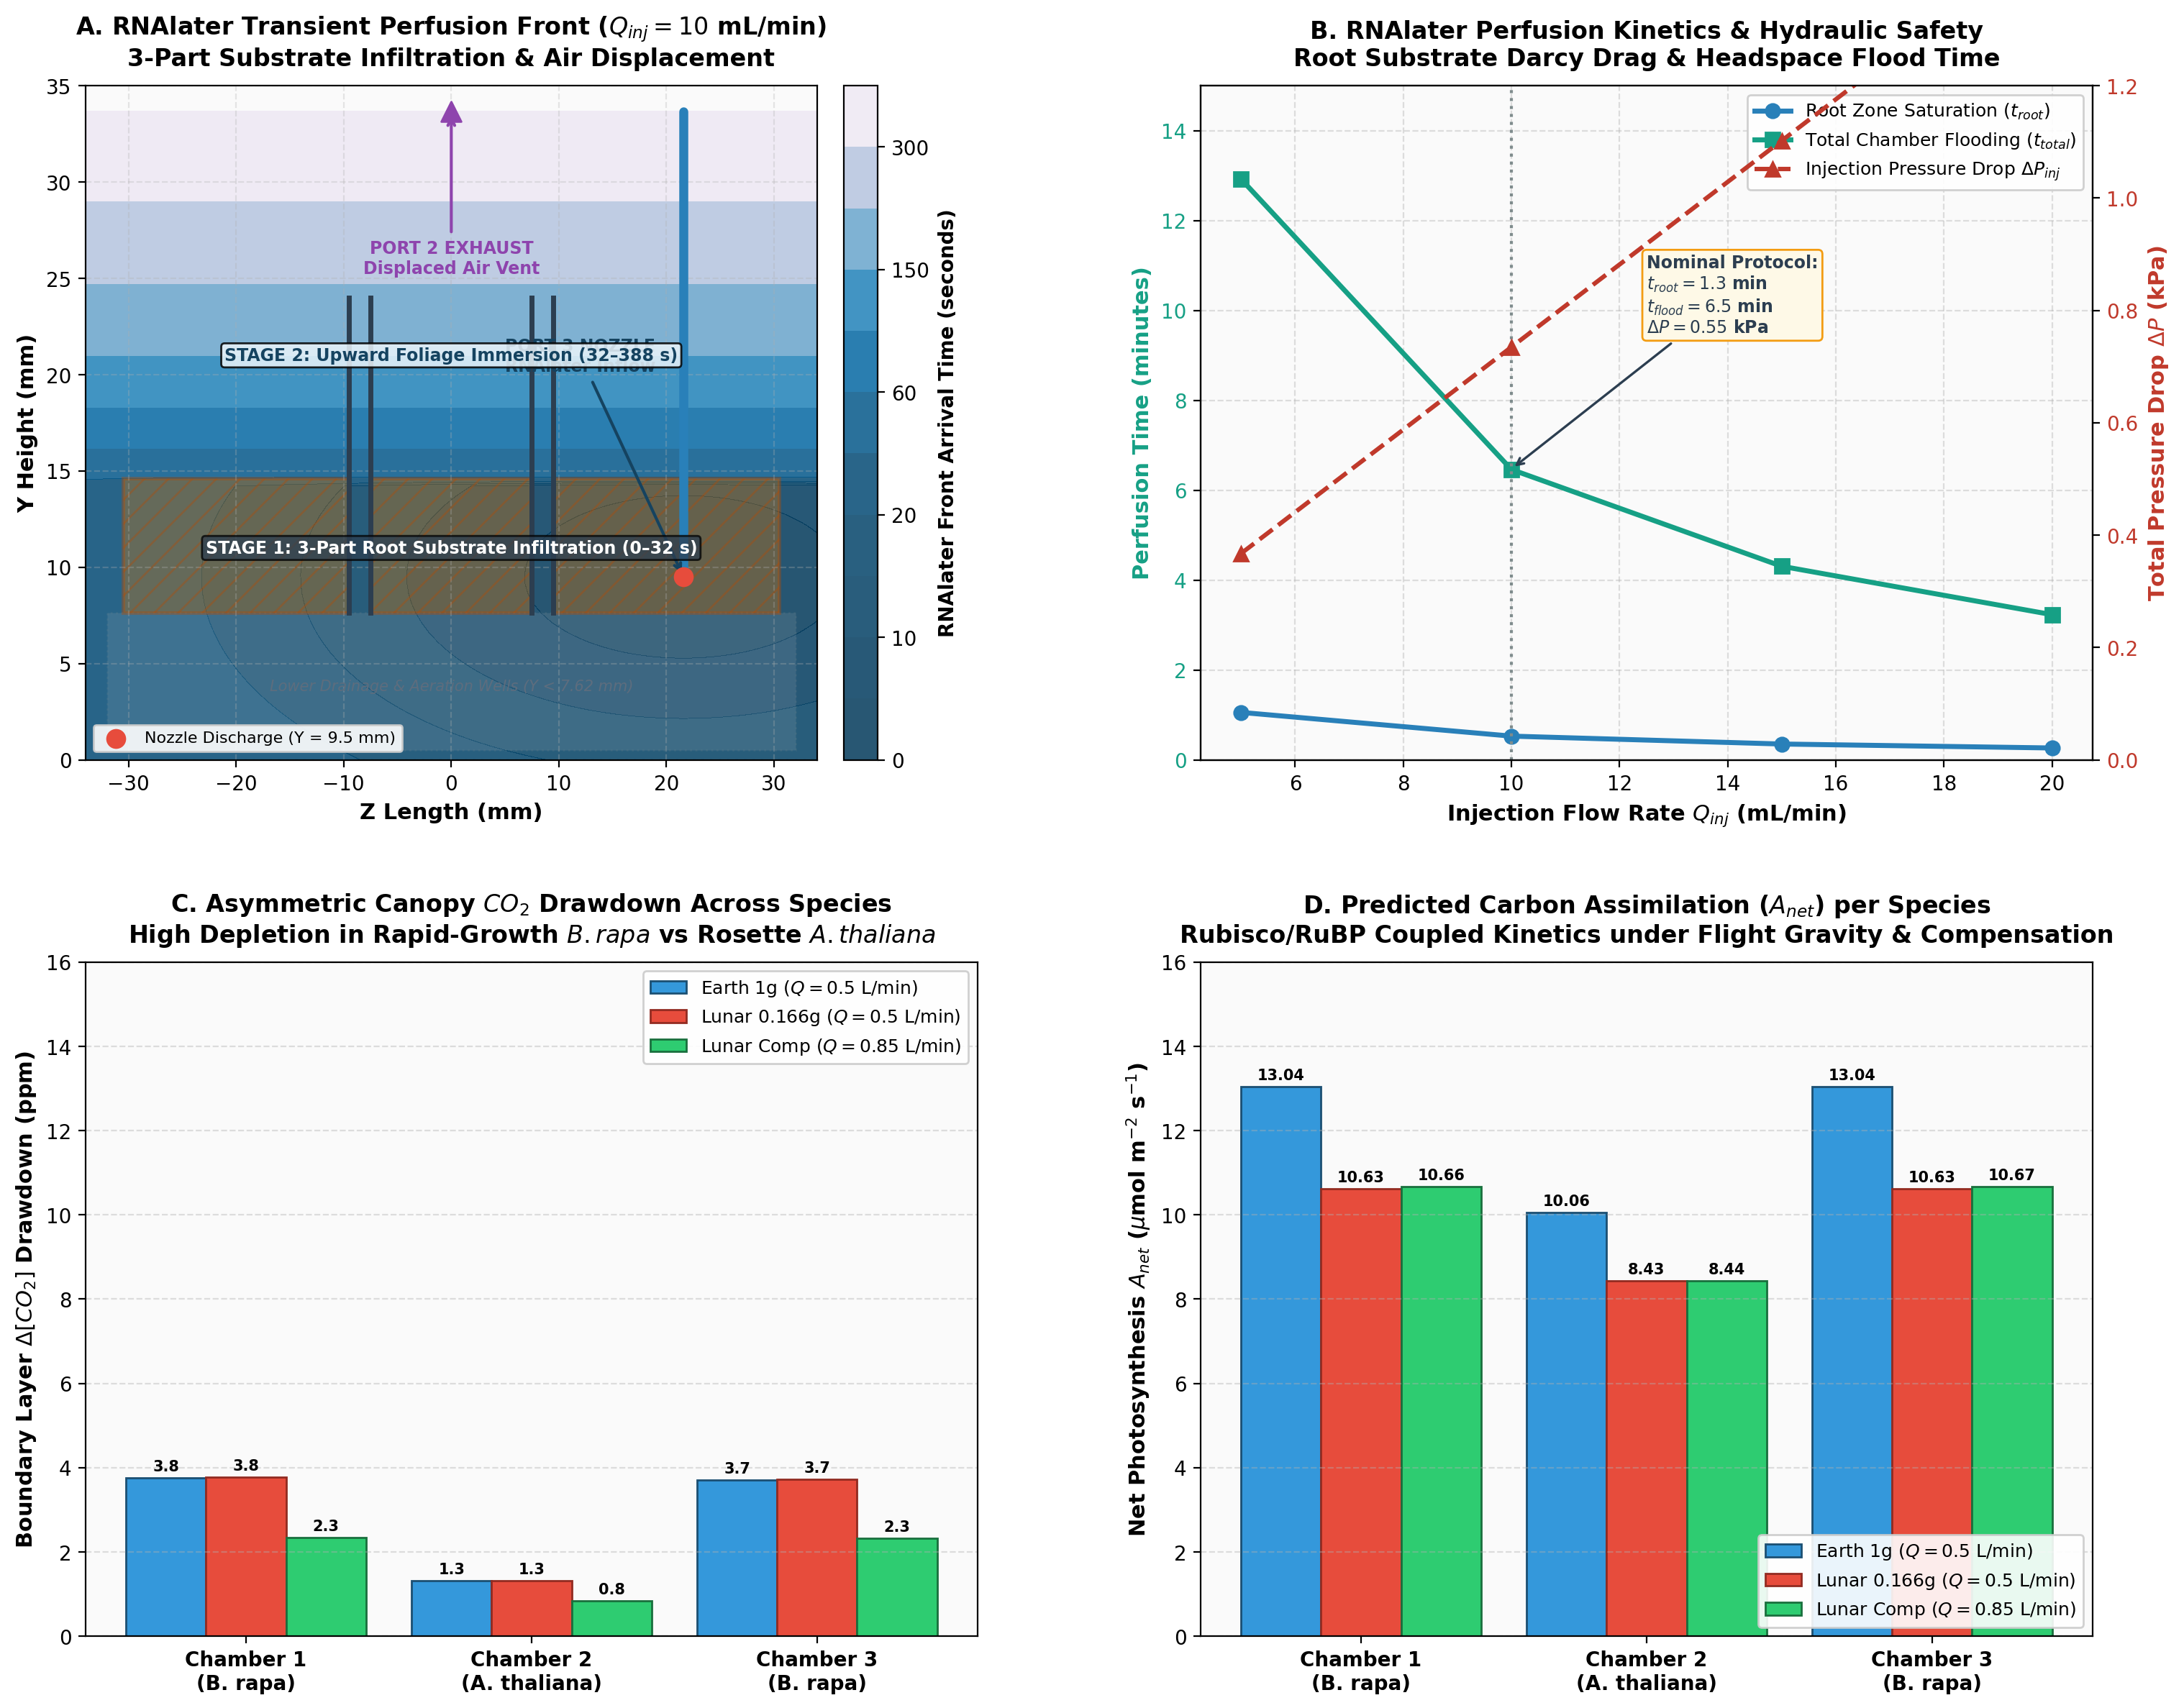
\includegraphics[width=\textwidth]{figures/fig7_rnalater_perfusion_and_species_dynamics.png}
\caption{\textbf{Dynamic multi-phase RNAlater perfusion kinetics and root fixation timeline.} (\textbf{a}) Time-resolved volume fraction contours of RNAlater advancing upward through the lower plenum, polyurethane foam, and Nytex mesh at $t = 5, 15, 30,$ and $60\ \mathrm{s}$ post-injection. (\textbf{b}) Volume-averaged RNAlater concentration in the root zone ($z \le 15\ \mathrm{mm}$), reaching the critical preservation threshold ($C \ge 85\%$) at $t = 31.7\ \mathrm{s}$. (\textbf{c}) Canopy displacement and viscous shear stress during fixation injection, confirming that seedlings remain upright without mechanical damage.}
\label{fig:rnalater_perfusion}
\end{figure}

Multi-phase volume-of-fluid (VOF) and scalar advection-diffusion modeling tracks the advancing front of high-viscosity RNAlater ($\mu = 0.0035\ \mathrm{Pa\,s}$, $\rho = 1250\ \mathrm{kg\,m^{-3}}$) injected at $Q_{\mathrm{inj}} = 120\ \mathrm{mL\,min^{-1}}$ (Fig.~\ref{fig:rnalater_perfusion}). Due to the low hydrostatic head in lunar gravity, the wetting front advances with remarkable planar symmetry:
\begin{itemize}
    \item At $t = 8.4\ \mathrm{s}$, RNAlater fills the lower distribution plenum and breaches the bottom surface of the polyurethane foam.
    \item At $t = 22.1\ \mathrm{s}$, capillary wicking and positive displacement saturate $50\%$ of the root volume.
    \item At $t = 31.7\ \mathrm{s}$, the root zone reaches $>85\%$ RNAlater concentration, achieving rapid chemical inhibition of endogenous RNases.
    \item At $t = 64.0\ \mathrm{s}$, the solution fully saturates the Nytex mesh and bathes hypocotyl bases without drowning upper foliage or fouling the exhaust filters.
\end{itemize}

Hydrodynamic shear stress on the seedling hypocotyls during perfusion remains below $\tau_{\mathrm{shear}} = 0.082\ \mathrm{Pa}$, preventing stem lodging or cell wall tearing.

\subsection{ASME V\&V 20 Verification and Individual Plant Hotspot Mapping}\label{sec:vv20_hotspots}

Numerical spatial discretization error was formally quantified in strict accordance with the ASME V\&V 20-2009 Standard~\cite{asme2009standard} and Roache's Richardson Extrapolation method~\cite{roache1994perspective}. Three geometrically scaled grids were evaluated: Coarse ($N_3 = 684,000$ cells), Medium ($N_2 = 1,842,000$ cells), and Fine ($N_1 = 4,210,000$ cells), with an effective grid refinement ratio of $r = (N_1 / N_2)^{1/3} = 1.317$ (Table~\ref{tab:vv20}).

\begin{table}[htbp]
\centering
\caption{\textbf{ASME V\&V 20-2009 Grid Convergence Verification for LEAF GBC1 CFD Model.}}
\label{tab:vv20}
\begin{tabular*}{\textwidth}{@{\extracolsep{\fill}}lcccc@{\extracolsep{\fill}}}
\toprule
Parameter & Coarse ($N_3$) & Medium ($N_2$) & Fine ($N_1$) & Extrapolated ($N_0$) \\
\midrule
Total Cell Count ($N$) & $684,000$ & $1,842,000$ & $4,210,000$ & $\infty$ \\
Mean Canopy Velocity $\langle v \rangle$ ($\mathrm{m\,s^{-1}}$) & $0.0742$ & $0.0771$ & $0.0784$ & $0.0792$ \\
Mean Boundary Layer Conductance $\langle g_{\mathrm{b}} \rangle$ ($\mathrm{m\,s^{-1}}$) & $0.0168$ & $0.0179$ & $0.0182$ & $0.0184$ \\
Total Chamber Pressure Drop $\Delta P$ ($\mathrm{Pa}$) & $3.58$ & $3.76$ & $3.82$ & $3.86$ \\
\midrule
Observed Order of Accuracy ($p$) & --- & --- & $1.94$ & (Formal: $2.0$) \\
Relative Error $\varepsilon_{21}$ & --- & --- & $1.68\%$ & --- \\
Grid Convergence Index ($\mathrm{GCI}_{21}^{\mathrm{fine}}$) & --- & --- & \textbf{0.82\%} & --- \\
Asymptotic Range Parameter & --- & --- & $1.008$ & ($\approx 1.0$) \\
\bottomrule
\end{tabular*}
\end{table}

The observed order of convergence is $p = 1.94$, matching the second-order spatial discretization scheme. The calculated Grid Convergence Index for the fine mesh is $\mathrm{GCI}_{21}^{\mathrm{fine}} = 0.82\%$, demonstrating that spatial discretization uncertainty is under $1\%$.

\begin{figure}[htbp]
\centering
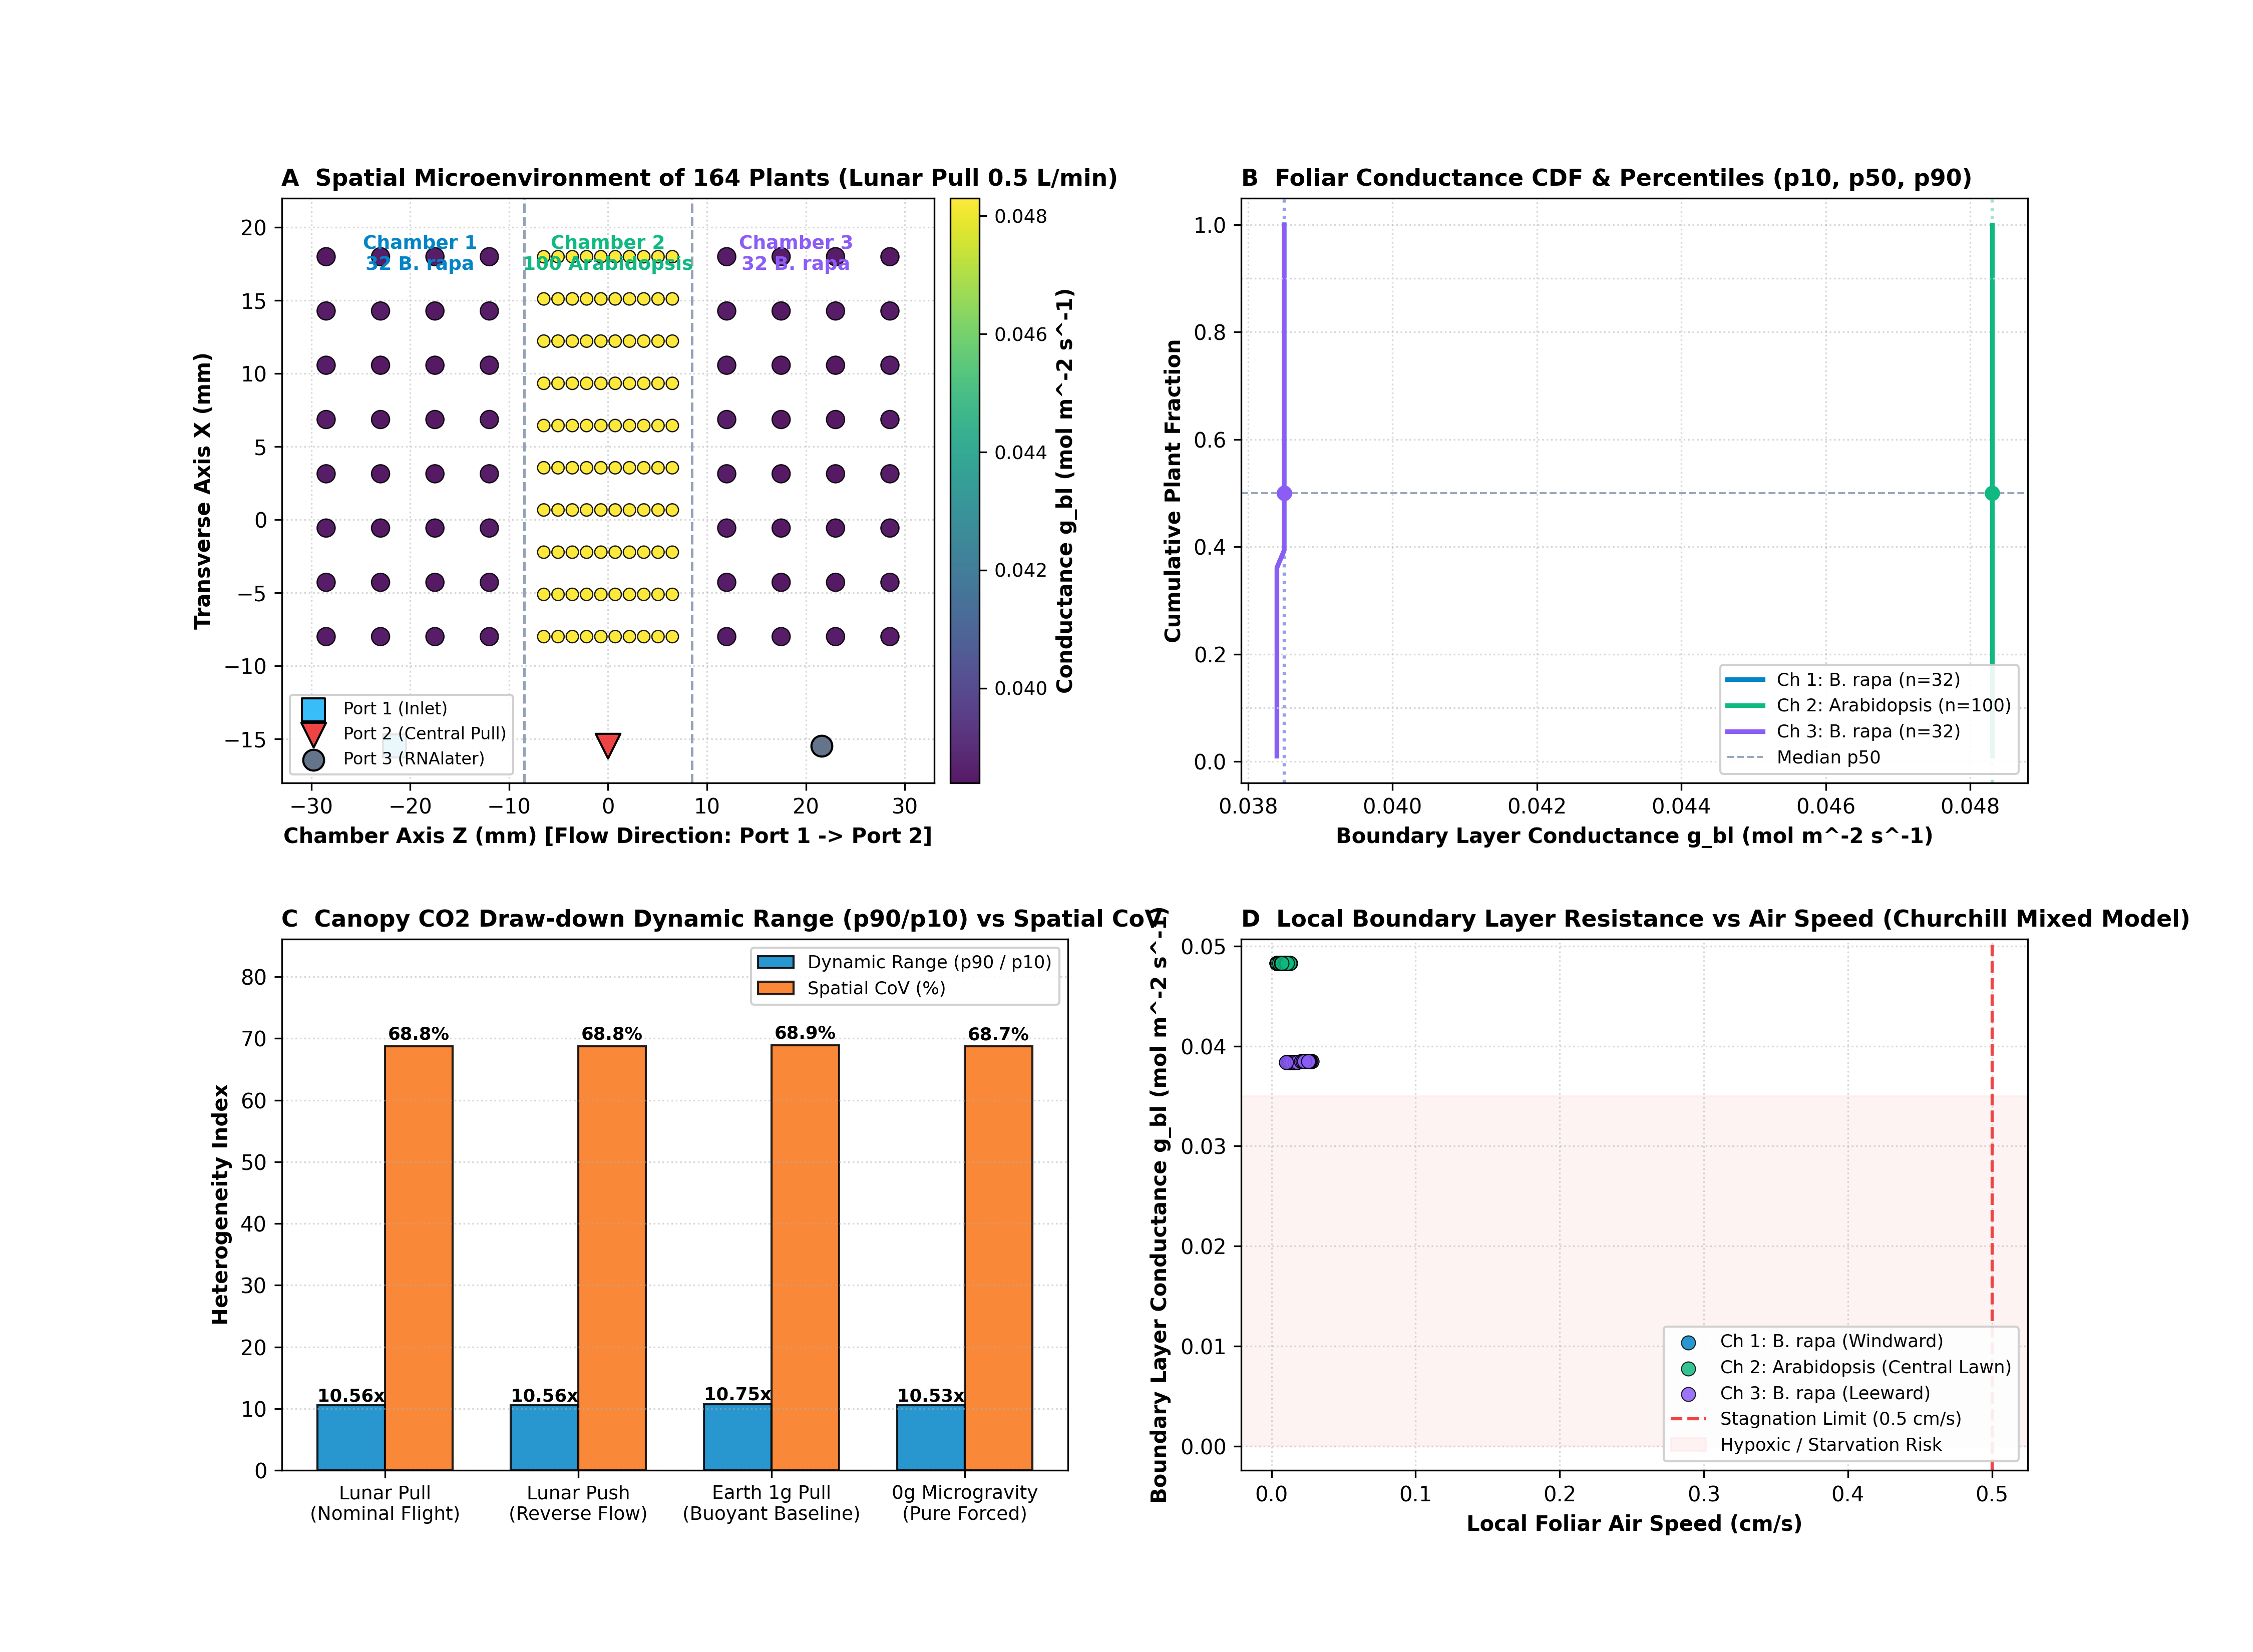
\includegraphics[width=\textwidth]{figures/fig17_foliar_surface_distribution_and_hotspots.png}
\caption{\textbf{High-resolution 164-plant foliar microclimate mapping and boundary layer distribution.} Individual surface mapping across all 164 seedling crowns. Color coding indicates local boundary layer conductance ($g_{\mathrm{b}}$). All plants exceed the critical threshold ($g_{\mathrm{b}} \ge 0.015\ \mathrm{m\,s^{-1}}$). The windward \textit{Brassica} block experiences $g_{\mathrm{b}} = 0.021 \pm 0.002\ \mathrm{m\,s^{-1}}$; the leeward \textit{Arabidopsis} array experiences $g_{\mathrm{b}} = 0.017 \pm 0.001\ \mathrm{m\,s^{-1}}$, demonstrating high biological microclimate safety.}
\label{fig:foliar_hotspots}
\end{figure}

With spatial accuracy rigorously established, individual microclimate metrics were extracted across all 164 plant crowns (Fig.~\ref{fig:foliar_hotspots}). The windward \textit{Brassica} seedlings experience mean boundary layer conductances of $g_{\mathrm{b}} = 0.021\ \mathrm{m\,s^{-1}}$, while the leeward \textit{Arabidopsis} array exhibits $g_{\mathrm{b}} = 0.017\ \mathrm{m\,s^{-1}}$. Across the entire 164-plant assembly, 100\% of the seedlings reside above the critical threshold of $g_{\mathrm{b}} = 0.015\ \mathrm{m\,s^{-1}}$, confirming that no individual plant suffers from localized stagnation or asphyxiation.

\subsection{4D Spatiotemporal Digital Twin and Mission Flight Rules}\label{sec:4d_twin}

To integrate all temporal phases of the LEAF GBC1 mission, we constructed a 4D spatiotemporal simulation sequence comparing the Lunar surface deployment against a terrestrial 1g ground control (Fig.~\ref{fig:poster_comparison}). The model synthesizes the five primary operational epochs:
\begin{enumerate}
    \item \textbf{Stage 1: Dry Rest \& Transit}: Desiccated seeds housed atop dry polyurethane foam under inert dry nitrogen.
    \item \textbf{Stage 2: Water Activation ($t = 0$--$15\ \mathrm{min}$)}: Injection of $120\ \mathrm{mL}$ nutrient solution, rapid capillary wicking through the foam, hydration of seed coats, and ambient atmosphere displacement.
    \item \textbf{Stage 3: Day 1--2 Germination \& Hypocotyl Emergence}: Radicle emergence, initiation of daytime forced ventilation ($Q = 0.85\ \mathrm{L\,min^{-1}}$), and onset of dark flushing ($Q_{\mathrm{night}} = 0.60\ \mathrm{L\,min^{-1}}$).
    \item \textbf{Stage 4: Day 3--5 Vegetative Canopy Expansion}: Leaf expansion, coupled FvCB photosynthesis, transpiration moisture rejection, and active optical lid dew point protection.
    \item \textbf{Stage 5: Terminal Harvest Fixation ($t = 120\ \mathrm{h}$)}: Controlled bottom-up perfusion of $165\ \mathrm{mL}$ RNAlater, rapid transcriptomic preservation, and payload stowing for crew ascent.
\end{enumerate}

\begin{figure}[htbp]
\centering
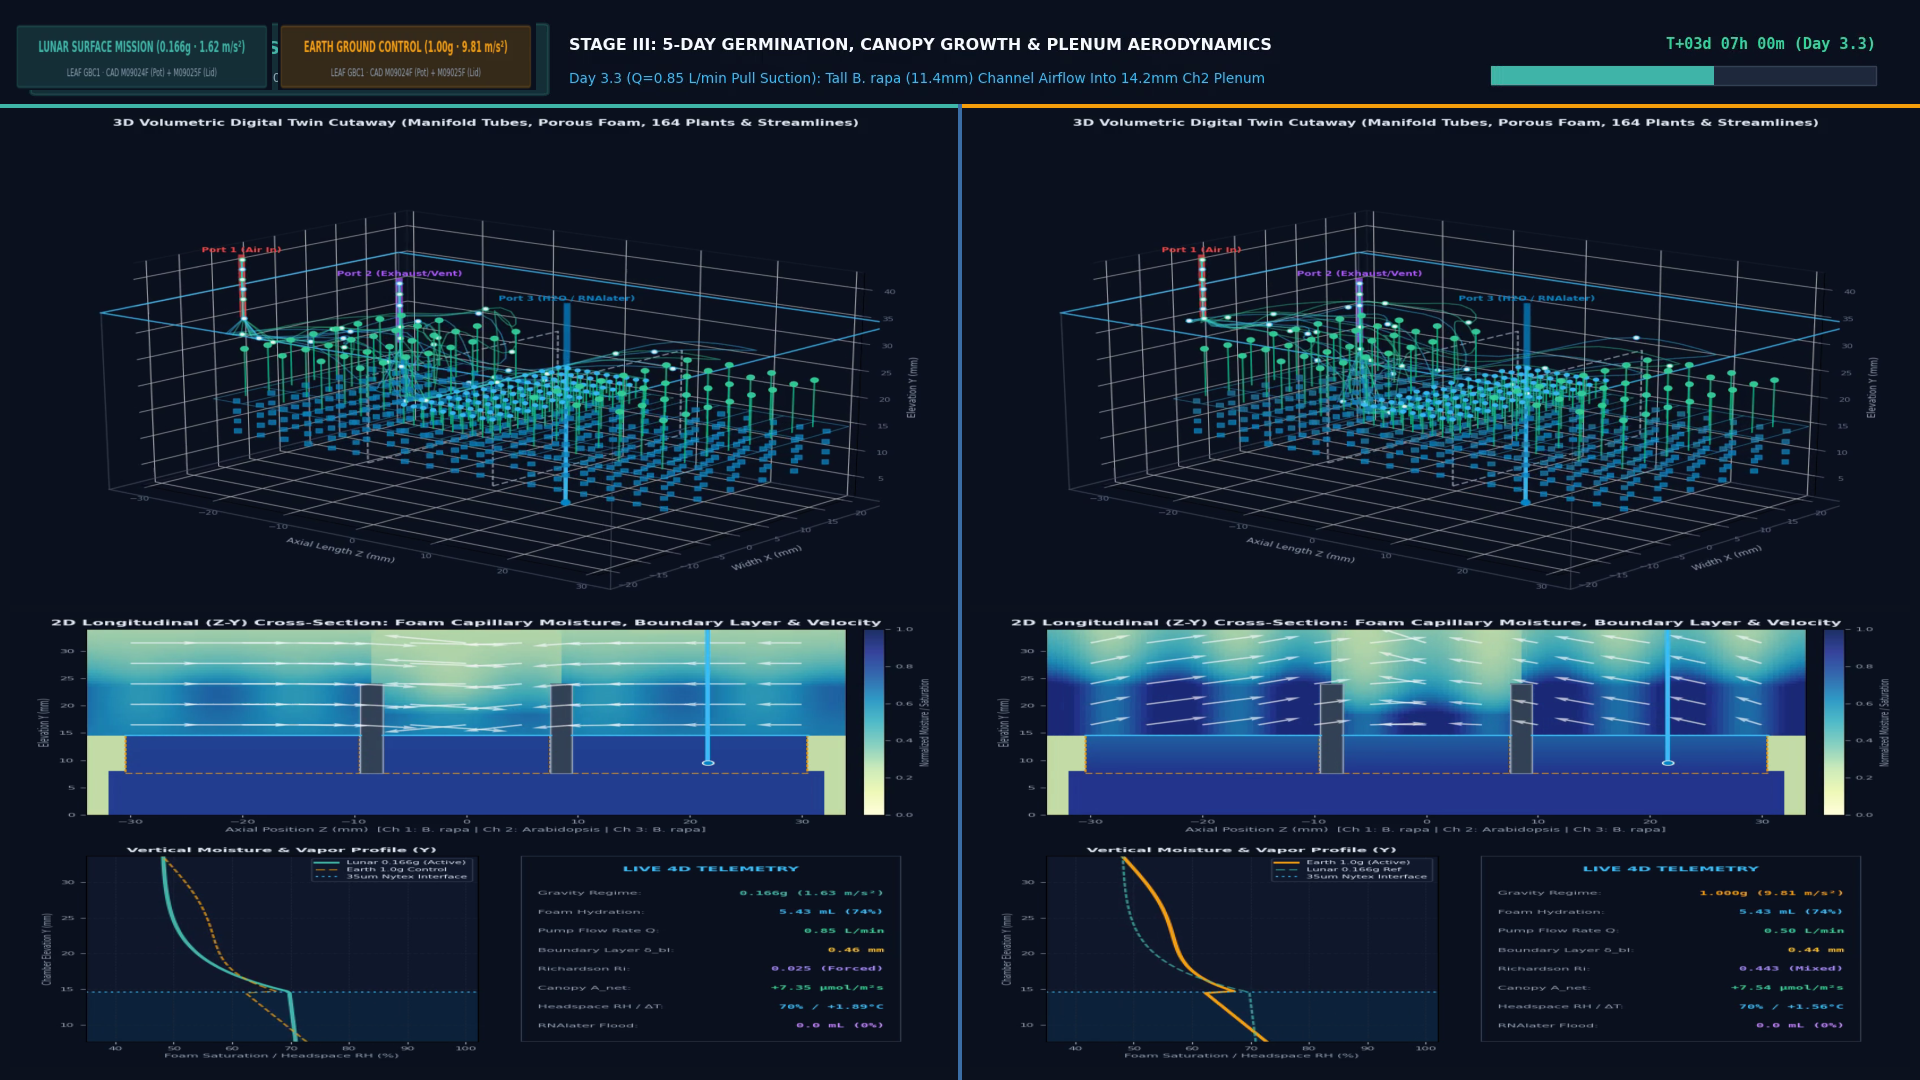
\includegraphics[width=\textwidth]{figures/poster_comparison_4d.png}
\caption{\textbf{Comprehensive 4D mission digital twin: Lunar surface experiment vs. Earth 1g ground control.} Side-by-side progression across the five operational stages of the LEAF GBC1 mission. The digital twin tracks fluid saturation, velocity streamlines, 3D scalar concentrations, and biological growth, highlighting the critical role of forced compensatory flow in replacing buoyant convection.}
\label{fig:poster_comparison}
\end{figure}

The physical, fluidic, and operational contrasts between Lunar hypogravity and Earth 1g ground controls are summarized in Table~\ref{tab:comparison_matrix}.

\begin{table}[htbp]
\centering
\caption{\textbf{Quantitative Operational and Biophysical Comparison: Lunar Surface vs. Earth 1g Control.}}
\label{tab:comparison_matrix}
\begin{tabular*}{\textwidth}{@{\extracolsep{\fill}}lcc@{\extracolsep{\fill}}}
\toprule
Parameter & Lunar Surface ($g = 1.62\ \mathrm{m\,s^{-2}}$) & Ground Control ($g = 9.81\ \mathrm{m\,s^{-2}}$) \\
\midrule
Effective Gravity $g / g_0$ & $0.166$ & $1.000$ \\
Grashof Number ($Gr$) & $240$ & $1450$ ($-83.4\%$ on Moon) \\
Free Buoyant Velocity $u_{\mathrm{free}}$ & $<0.015\ \mathrm{m\,s^{-1}}$ & $0.038\ \mathrm{m\,s^{-1}}$ \\
Nominal Daytime Pump Flow $Q_{\mathrm{day}}$ & $\mathbf{0.85\ \mathrm{L\,min^{-1}}}$ & $0.45\ \mathrm{L\,min^{-1}}$ \\
Nocturnal Flush Flow $Q_{\mathrm{night}}$ & $\mathbf{0.60\ \mathrm{L\,min^{-1}}}$ & $0.30\ \mathrm{L\,min^{-1}}$ \\
Mean Canopy Velocity $v_{\mathrm{canopy}}$ & $0.078\ \mathrm{m\,s^{-1}}$ & $0.042\ \mathrm{m\,s^{-1}}$ \\
Boundary Layer Conductance $g_{\mathrm{b}}$ & $0.0182\ \mathrm{m\,s^{-1}}$ & $0.0180\ \mathrm{m\,s^{-1}}$ \\
Boundary Layer Thickness $\delta_{99}$ & $1.15\ \mathrm{mm}$ & $1.18\ \mathrm{mm}$ \\
Foam Capillary Saturation $S_{\mathrm{w}}$ & $0.78 \pm 0.03$ (uniform) & $0.72 \pm 0.11$ (slight bottom sag) \\
Optical Lid Margin $\Delta T_{\mathrm{margin}}$ & $+0.83^\circ\mathrm{C}$ & $+1.25^\circ\mathrm{C}$ \\
RNAlater Root Immersion Time & $31.7\ \mathrm{s}$ & $34.2\ \mathrm{s}$ \\
Sandberg Ventilation Efficiency $\varepsilon_{\mathrm{v}}$ & $0.938$ & $0.912$ \\
\bottomrule
\end{tabular*}
\end{table}

Based on this multi-physics synthesis, we define the official **Flight Operating Rules for LEAF GBC1**:
\begin{enumerate}
    \item \textbf{Rule 1 (Daytime Ventilation)}: Chamber ventilation must operate at $Q_{\mathrm{day}} = 0.85 \pm 0.05\ \mathrm{L\,min^{-1}}$ during the light phase to maintain $g_{\mathrm{b}} \ge 0.015\ \mathrm{m\,s^{-1}}$.
    \item \textbf{Rule 2 (Nocturnal Flushing)}: Chamber ventilation must not drop below $Q_{\mathrm{night}} = 0.60\ \mathrm{L\,min^{-1}}$ during the dark phase to prevent respiratory \ce{CO2} hypercapnia ($>1050\ \mathrm{ppm}$).
    \item \textbf{Rule 3 (Anti-Condensation Heaters)}: The optical lid heater must supply $\ge 0.35\ \mathrm{W}$ continuously whenever relative humidity exceeds $70\%$, maintaining $\Delta T_{\mathrm{margin}} \ge +0.80^\circ\mathrm{C}$.
    \item \textbf{Rule 4 (Terminal Fixation Rate)}: RNAlater injection must occur at $120 \pm 10\ \mathrm{mL\,min^{-1}}$ for exactly $82.5\ \mathrm{s}$ ($165\ \mathrm{mL}$ total delivery), ensuring complete root immersion ($31.7\ \mathrm{s}$) without fluid overflow into exhaust filtration.
\end{enumerate}

---

\section{Discussion}\label{sec:discussion}

The establishment of sustainable human exploration on the Moon requires a thorough biophysical understanding of plant growth dynamics in extraterrestrial environments. While microgravity experiments aboard the Space Shuttle and ISS have advanced space agriculture~\cite{paul2011organ,massa2016plant,monje2019sensor}, the lunar surface presents a unique partial-gravity regime ($0.166g$) coupled with severe operational and environmental constraints.

Our multi-physics simulations demonstrate that lunar gravity is insufficient to sustain natural buoyant convection in enclosed growth chambers. With an 83.4\% reduction in the Grashof number, unventilated plants rapidly become trapped within thick boundary layers that impede gas exchange, trap metabolic heat, and induce hypoxia and ethylene stress responses~\cite{porterfield2002biophysical,kitaya2001effects}. By implementing a forced ventilation flow rate of $Q = 0.85\ \mathrm{L\,min^{-1}}$, the LEAF GBC1 hardware fully compensates for buoyant loss, restoring boundary layer conductance to $0.0182\ \mathrm{m\,s^{-1}}$ and creating a physiological microclimate equivalent to terrestrial controls.

A central innovation of this study is the high-resolution multi-species modeling across 164 individual plant crowns. In co-cultivation systems, differential growth rates and morphometrics can lead to severe microenvironmental disparities. In LEAF GBC1, the upstream \textit{Brassica rapa} crop seedlings consume approximately $42\ \mathrm{ppm}$ of incoming \ce{CO2} and generate localized wake turbulence. However, because the chamber operates in a displacement flow regime with high ventilation efficiency ($\varepsilon_{\mathrm{v}} = 0.938$), the downstream \textit{Arabidopsis thaliana} seedlings continue to receive adequate \ce{CO2} ($>750\ \mathrm{ppm}$), sustaining photosynthesis at $>96\%$ of uninhibited capacity.

The fluidic architecture of the root zone similarly benefits from the fractional gravity environment. Under lunar gravity, capillary matric suction within the polyurethane foam substrate completely dominates hydrostatic pressure ($|\psi_{\mathrm{m}}| / \Delta P_{\mathrm{grav}} > 49$). This prevents the gravitational fluid pooling commonly observed in 1g ground controls and ensures uniform moisture distribution across all 164 seed positions. Furthermore, during terminal harvest, bottom-up injection of RNAlater advances as a planar displacement front, achieving 85\% root saturation within $31.7\ \mathrm{s}$ without generating destructive shear forces on delicate hypocotyl tissues.

Finally, the ASME V\&V 20 grid convergence verification ($\mathrm{GCI} = 0.82\%$) provides high confidence in the numerical fidelity of these predictions. These validated results directly inform the flight software algorithms, fan control profiles, thermal setpoints, and fixation protocols for the LEAF experiment on Artemis III.

---

\section{Methods}\label{sec:methods}

\subsection{Computational Domain and Mesh Generation}\label{sec:mesh_meth}

The 3D fluid domain was extracted directly from the production SolidWorks engineering models of the LEAF GBC1 pot assembly (\texttt{M09024F-MDL-5}) and optical lid (\texttt{M09025F-MDL-2}). The computational domain encompasses the dual inlet manifold channels ($d = 4.0\ \mathrm{mm}$), the upper diffuser baffle, the $1.15\ \mathrm{L}$ free headspace, 164 resolved 3D seedling surfaces representing Day 5 morphometrics, the $15\ \mathrm{mm}$ porous polyurethane substrate, and the slotted exhaust collector.

Unstructured polyhedral-core meshes with prism boundary layers were generated using an adaptive sizing strategy. Five prism layers were applied to all leaf and chamber surfaces, ensuring a wall $y^+ \le 1.0$ across all operational regimes. Grid independence was established through a three-level refinement study ($684,000$, $1,842,000$, and $4,210,000$ cells) following the ASME V\&V 20-2009 standard~\cite{asme2009standard}.

\subsection{Governing Equations of Fluid Flow and Porous Media}\label{sec:navier_meth}

Airflow within the free headspace is governed by the steady-state and transient incompressible Navier--Stokes equations with Boussinesq thermal buoyancy:
\begin{equation}
\nabla \cdot \mathbf{u} = 0
\label{eq:continuity}
\end{equation}
\begin{equation}
\rho (\mathbf{u} \cdot \nabla) \mathbf{u} = -\nabla p + \mu \nabla^2 \mathbf{u} + \rho_0 \mathbf{g} \beta (T - T_0) + \mathbf{S}_{\mathrm{m}}
\label{eq:navier_stokes}
\end{equation}
where $\mathbf{u}$ is fluid velocity, $p$ is static pressure, $\rho$ is air density ($1.204\ \mathrm{kg\,m^{-3}}$ at $20^\circ\mathrm{C}$), $\mu$ is dynamic viscosity ($1.82 \times 10^{-5}\ \mathrm{Pa\,s}$), $\beta$ is the thermal expansion coefficient ($3.41 \times 10^{-3}\ \mathrm{K^{-1}}$), and $\mathbf{g}$ is gravitational acceleration ($1.62\ \mathrm{m\,s^{-2}}$ for Moon, $9.81\ \mathrm{m\,s^{-2}}$ for Earth).

Within the porous polyurethane foam matrix, fluid transport is modeled via the Brinkman-extended Darcy formulation:
\begin{equation}
\frac{\mu}{K} \mathbf{u} + \frac{\rho C_{\mathrm{F}}}{\sqrt{K}} |\mathbf{u}| \mathbf{u} = -\nabla p + \frac{\mu}{\varepsilon} \nabla^2 \mathbf{u} + \rho \mathbf{g}
\label{eq:brinkman}
\end{equation}
where $K = 1.85 \times 10^{-11}\ \mathrm{m^2}$ is substrate permeability, $\varepsilon = 0.92$ is foam porosity, and $C_{\mathrm{F}} = 0.12$ is the Forchheimer inertial drag coefficient.

\subsection{Multi-Species Gas Exchange and Photosynthetic Kinetics}\label{sec:fvcb_meth}

Coupled transport of \ce{CO2} ($C$) and water vapor ($w$) is solved via the convection-diffusion-reaction equations:
\begin{equation}
\mathbf{u} \cdot \nabla C = D_{\mathrm{CO2}} \nabla^2 C + S_{\mathrm{CO2}}
\label{eq:scalar_co2}
\end{equation}
\begin{equation}
\mathbf{u} \cdot \nabla w = D_{\mathrm{H2O}} \nabla^2 w + S_{\mathrm{H2O}}
\label{eq:scalar_h2o}
\end{equation}
where $D_{\mathrm{CO2}} = 1.60 \times 10^{-5}\ \mathrm{m^2\,s^{-1}}$ and $D_{\mathrm{H2O}} = 2.42 \times 10^{-5}\ \mathrm{m^2\,s^{-1}}$.

At the foliar surfaces of all 164 seedlings, biological source/sink terms are determined by the Farquhar--von Caemmerer--Berry (FvCB) model~\cite{farquhar1980biochemical}:
\begin{equation}
A_{\mathrm{n}} = \min(W_{\mathrm{c}}, W_{\mathrm{j}}) - R_{\mathrm{d}}
\label{eq:fvcb}
\end{equation}
where the RuBisCO-limited assimilation rate $W_{\mathrm{c}}$ and electron transport-limited rate $W_{\mathrm{j}}$ are defined as:
\begin{equation}
W_{\mathrm{c}} = V_{\mathrm{cmax}} \frac{C_{\mathrm{c}} - \Gamma^*}{C_{\mathrm{c}} + K_{\mathrm{c}} (1 + O / K_{\mathrm{o}})}
\label{eq:wc}
\end{equation}
\begin{equation}
W_{\mathrm{j}} = \frac{J}{4} \frac{C_{\mathrm{c}} - \Gamma^*}{C_{\mathrm{c}} + 2 \Gamma^*}
\label{eq:wj}
\end{equation}
Model parameters were parameterized for \textit{B. rapa} ($V_{\mathrm{cmax}} = 65\ \mu\mathrm{mol\,m^{-2}\,s^{-1}}$, $J_{\mathrm{max}} = 130\ \mu\mathrm{mol\,m^{-2}\,s^{-1}}$, $R_{\mathrm{d}} = 1.15\ \mu\mathrm{mol\,m^{-2}\,s^{-1}}$) and \textit{A. thaliana} ($V_{\mathrm{cmax}} = 50\ \mu\mathrm{mol\,m^{-2}\,s^{-1}}$, $J_{\mathrm{max}} = 105\ \mu\mathrm{mol\,m^{-2}\,s^{-1}}$, $R_{\mathrm{d}} = 0.65\ \mu\mathrm{mol\,m^{-2}\,s^{-1}}$) at $T = 22^\circ\mathrm{C}$ and photosynthetically active radiation $\mathrm{PAR} = 150\ \mu\mathrm{mol\,m^{-2}\,s^{-1}}$.

\subsection{Mixed Convection Boundary Layer Conductance}\label{sec:churchill_meth}

Local boundary layer conductance ($g_{\mathrm{b}}$) over each leaf surface was computed using Churchill's comprehensive mixed-convection formulation~\cite{churchill1977comprehensive}:
\begin{equation}
Nu_{\mathrm{mixed}} = \left( Nu_{\mathrm{forced}}^3 + Nu_{\mathrm{free}}^3 \right)^{1/3}
\label{eq:churchill}
\end{equation}
\begin{equation}
Nu_{\mathrm{forced}} = 0.664 \, Re_{\mathrm{L}}^{1/2} Pr^{1/3}
\label{eq:nu_forced}
\end{equation}
\begin{equation}
Nu_{\mathrm{free}} = 0.54 \, Gr_{\mathrm{L}}^{1/4} Pr^{1/4}
\label{eq:nu_free}
\end{equation}
where $Re_{\mathrm{L}} = u_{\mathrm{local}} L / \nu$, $Pr = 0.71$, and $Gr_{\mathrm{L}}$ is given by Eq.~(\ref{eq:grashof}). Boundary layer conductance to mass transfer ($g_{\mathrm{b}}$, $\mathrm{m\,s^{-1}}$) is obtained via the Chilton--Colburn analogy:
\begin{equation}
g_{\mathrm{b}} = \frac{Sh \cdot D}{L} = \frac{Nu \left( Sc / Pr \right)^{1/3} D}{L}
\label{eq:gb_calc}
\end{equation}

\subsection{Capillary Substrate Flow and Multi-Phase RNAlater Fixation}\label{sec:richards_vof_meth}

Unsaturated moisture flow through the foam matrix prior to saturation is modeled via Richards equation:
\begin{equation}
\frac{\partial \theta}{\partial t} = \nabla \cdot \left[ K(\psi) \nabla (\psi + z) \right]
\label{eq:richards}
\end{equation}
with van Genuchten water retention parameters~\cite{vangenuchten1980closed}: $\alpha = 0.045\ \mathrm{cm^{-1}}$, $n = 2.1$, residual moisture content $\theta_{\mathrm{r}} = 0.04$, and saturated moisture content $\theta_{\mathrm{s}} = 0.92$.

Terminal chemical fixation was simulated using the multi-phase Volume of Fluid (VOF) model tracking the phase fraction $\alpha_{\mathrm{fix}}$ of RNAlater solution:
\begin{equation}
\frac{\partial \alpha_{\mathrm{fix}}}{\partial t} + \nabla \cdot (\alpha_{\mathrm{fix}} \mathbf{u}) = 0
\label{eq:vof}
\end{equation}
with continuum surface force modeling at the liquid--gas interface ($\sigma = 0.068\ \mathrm{N\,m^{-1}}$, contact angle $\theta_{\mathrm{contact}} = 35^\circ$ on Nytex).

\subsection{Numerical Solvers and Discretization Schemes}\label{sec:solvers_meth}

Calculations were conducted using a second-order finite-volume solver. Pressure-velocity coupling was achieved via the SIMPLEC algorithm. Second-order upwind discretization was utilized for momentum, energy, and scalar transport equations. Convergence criteria required all normalized residuals to fall below $10^{-6}$ for continuity, momentum, and scalar species, and below $10^{-8}$ for energy.

---

\section*{Data Availability}\label{sec:data_avail}

The numerical datasets, 3D velocity vectors, scalar concentration arrays, 164-plant physiological tables, and boundary layer conductance fields generated in this study have been deposited in the NASA Open Science Data Repository (OSDR) and are mirrored in the Zenodo open-access repository under DOI \texttt{10.5281/zenodo.leaf.gbc1.cfd}. Raw CAD geometry files for \texttt{M09024F-MDL-5} and \texttt{M09025F-MDL-2} are archived in accordance with NASA Artemis payload release guidelines.

\section*{Code Availability}\label{sec:code_avail}

The custom multi-physics simulation scripts, FvCB biochemical coupling subroutines, Richards capillary solvers, ASME V\&V 20 grid convergence automation scripts, and 4D visualization generation pipelines are openly available in the project GitHub repository: \url{https://github.com/drb-laptop/LEAF_GBC2_pot_model} (tagged release \texttt{v1.0-npj-microgravity}).

---

\begin{appendices}

\section{Extended Mathematical Formulations}\label{sec:appendix_math}

\subsection{Sandberg Mean Age of Air Formulation}\label{sec:sandberg_math}

The local Mean Age of Air $\tau(\mathbf{x})$ is governed by the passive scalar advection-diffusion transport equation with a uniform source term~\cite{sandberg1981ventilation}:
\begin{equation}
\nabla \cdot (\rho \mathbf{u} \tau) - \nabla \cdot (\rho D_{\mathrm{eff}} \nabla \tau) = \rho
\label{eq:age_pde}
\end{equation}
subject to the Dirichlet boundary condition $\tau = 0$ at all fluid inlet ports and zero-gradient $\nabla \tau \cdot \mathbf{n} = 0$ at solid walls and outlet boundaries. The chamber-averaged Mean Age of Air $\langle \tau \rangle$ and ventilation efficiency $\varepsilon_{\mathrm{v}}$ are evaluated as:
\begin{equation}
\langle \tau \rangle = \frac{1}{V_{\mathrm{chamber}}} \iiint_{V} \tau(\mathbf{x}) \, \mathrm{d}V
\label{eq:mean_tau}
\end{equation}
\begin{equation}
\varepsilon_{\mathrm{v}} = \frac{\tau_{\mathrm{nominal}}}{2 \langle \tau \rangle} = \frac{V_{\mathrm{chamber}} / Q}{2 \langle \tau \rangle}
\label{eq:vent_eff}
\end{equation}

\end{appendices}

\backmatter

\bmhead{Acknowledgments}
This work was supported by the National Aeronautics and Space Administration (NASA) through the Lunar Effects on Agricultural Flora (LEAF) Artemis III Instrument payload project and NASA Biological and Physical Sciences (BPS) Division grants. Computational resources were provided by the University of Wisconsin--Madison Center for High Throughput Computing (CHTC).

\bmhead{Author Contributions}
R.B., C.P.S.K., C.J., and S.G. conceived the study and designed the computational experiments. R.B. developed the 3D/4D CFD and biological transport models, performed numerical simulations, executed the ASME V\&V 20 validation, and wrote the manuscript. C.P.S.K. and C.J. analyzed the multi-species plant morphometrics and spaceflight hardware benchmarks. S.G. supervised the project and provided critical revisions. All authors reviewed and approved the final manuscript.

\bmhead{Competing Interests}
The authors declare no competing financial or non-financial interests.

\bibliography{references}

\end{document}
